% ******************************* PhD Thesis Template **************************
\documentclass[a4paper,12pt,numbered,print,customfont,oneside]{PhDThesisPSnPDF}


% ******************************************************************************
% ******************************* Class Options ********************************
% *********************** See README for more details **************************
% ******************************************************************************

% `a4paper'(The University of Cambridge PhD thesis guidelines recommends a page
% size a4 - default option) or `a5paper': A5 Paper size is also allowed as per
% the Cambridge University Engineering Deparment guidelines for PhD thesis
%
% `11pt' or `12pt'(default): Font Size 10pt is NOT recommended by the University
% guidelines
%
% `oneside' or `twoside'(default): Printing double side (twoside) or single
% side.
%
% `print': Use `print' for print version with appropriate margins and page
% layout. Leaving the options field blank will activate Online version.
%
% `index': For index at the end of the thesis
%
% `draftclassic': For draft mode without loading any images (same as draft in book)
%
% `draft': Special draft mode with line numbers, images, and water mark with
% timestamp and custom text. Position of the text can also be modified.
%
% `abstract': To generate only the title page and abstract page with
% dissertation title and name, to submit to the Student Registry
%
% `chapter`: This option enables only the specified chapter and it's references
%  Useful for review and corrections.
%
% ************************* Custom Page Margins ********************************
%
% `custommargin`: Use `custommargin' in options to activate custom page margins,
% which can be defined in the preamble.tex. Custom margin will override
% print/online margin setup.
%
% *********************** Choosing the Fonts in Class Options ******************
%
% `times' : Times font with math support. 
%
% `fourier': Utopia Font with Fourier Math font (Font has to be installed)
%            It's a free font.
%
% `customfont': Use `customfont' option in the document class and load the
% package in the preamble.tex
%
% default or leave empty: `Latin Modern' font will be loaded.
%
% ********************** Choosing the Bibliography style ***********************
%
% `authoryear': For author-year citation eg., Smith (2013)
%
% `numbered': (Default Option) For numbered and sorted citation e.g., [1,5,2]
%
% `custombib': Define your own bibliography style in the `preamble.tex' file.
%              `\RequirePackage[square, sort, numbers, authoryear]{natbib}'.
%              This can be also used to load biblatex instead of natbib
%              (See Preamble)
%
% **************************** Choosing the Page Style *************************
%
% `default (leave empty)': For Page Numbers in Header (Left Even, Right Odd) and
% Chapter Name in Header (Right Even) and Section Name (Left Odd). Blank Footer.
%
% `PageStyleI': Chapter Name next & Page Number on Even Side (Left Even).
% Section Name & Page Number in Header on Odd Side (Right Odd). Footer is empty.
%
% `PageStyleII': Chapter Name on Even Side (Left Even) in Header. Section Number
% and Section Name in Header on Odd Side (Right Odd). Page numbering in footer

% Uncomment to change page style
\pagestyle{PageStyleII}

% ********************************** Preamble **********************************
% Preamble: Contains packages and user-defined commands and settings
% ******************************************************************************
% ****************************** Custom Margin *********************************

% Add `custommargin' in the document class options to use this section
% Set {innerside margin / outerside margin / topmargin / bottom margin}  and
% other page dimensions
\ifsetCustomMargin
  \RequirePackage[left=37mm,right=30mm,top=35mm,bottom=30mm]{geometry}
  \setFancyHdr % To apply fancy header after geometry package is loaded
\fi

% Add spaces between paragraphs
%\setlength{\parskip}{0.5em}
% Ragged bottom avoids extra whitespaces between paragraphs
\raggedbottom
% To remove the excess top spacing for enumeration, list and description
%\usepackage{enumitem}
%\setlist[enumerate,itemize,description]{topsep=0em}

% *****************************************************************************
% ******************* Fonts (like different typewriter fonts etc.)*************
\usepackage{rotating}
\usepackage{pdflscape}

\usepackage{booktabs,array,ragged2e}
\newcommand{\vname}[1]{\mathrm{#1}} % or: \mathit
\def\sectionautorefname{Section}
\def\subsectionautorefname{Section}
\def\subsubsectionautorefname{Section}
% At best in the preamble:
\DeclareRobustCommand\mytikzdot{\tikz \fill[black] (1ex,1ex) circle (0.5ex);}
\DeclareRobustCommand\mytikzreddot{\tikz \fill[red] (1ex,1ex) circle (0.5ex);}
\DeclareRobustCommand\mytikzbluedot{\tikz \fill[blue] (1ex,1ex) circle (0.5ex);}
% Add `customfont' in the document class option to use this section
%\usepackage{mathtools}
\ifsetCustomFont
%\usepackage{mathtools}
%
%\usepackage[T1]{fontenc}
\usepackage{lmodern}
\newcommand\hmmax{0}
\newcommand\bmmax{0}
%\usepackage[T1]{fontenc}
%\usepackage[notextcomp]{kpfonts}%  for math    
%\usepackage{libertine}%  serif and sans serif
%\usepackage[scaled=0.85]{beramono}%% mono
\usepackage[T1]{fontenc}
\usepackage{newpxtext}% FOR PALATINO TEXT
\usepackage{newpxmath}% FOR MATH
%\RequirePackage{mathpazo} % Palatino with real small caps and old style figures
%\PassOptionsToPackage[osf,sc]{mathpazo}%
%\usepackage[osf,sc]{mathpazo}%
%\usepackage{newpxtext}
\usepackage{newpxmath}
\usepackage{notoccite}% PREVENTS CITES IN CAPTIONS FROM MISNUMBERING YOUR REFERENCES 

%\linespread{1.25} % a bit more for Palatino
\usepackage{bm}
\usepackage{setspace}

\usepackage{enumerate}% http://ctan.org/pkg/enumerate

\usepackage{braket}
\usepackage{makecell}
\usepackage{xspace}

\newcommand*{\vecc}[1]{%
	\if#1\relax\bm{#1}\else\mathbf{#1}\fi
}

%\linespread{1.05} % a bit more for Palatino
  % Set your custom font here and use `customfont' in options. Leave empty to
  % load computer modern font (default LaTeX font).
  %\RequirePackage{helvet}

  % For use with XeLaTeX
  %  \setmainfont[
  %    Path              = ./libertine/opentype/,
  %    Extension         = .otf,
  %    UprightFont = LinLibertine_R,
  %    BoldFont = LinLibertine_RZ, % Linux Libertine O Regular Semibold
  %    ItalicFont = LinLibertine_RI,
  %    BoldItalicFont = LinLibertine_RZI, % Linux Libertine O Regular Semibold Italic
  %  ]
  %  {libertine}
  %  % load font from system font
  %  \newfontfamily\libertinesystemfont{Linux Libertine O}
\fi


%



% *****************************************************************************
% **************************** Custom Packages ********************************

% ************************* Algorithms and Pseudocode **************************

%\usepackage{algpseudocode}


% ********************Captions and Hyperreferencing / URL **********************

% Captions: This makes captions of figures use a boldfaced small font.
%\RequirePackage[small,bf]{caption}

\RequirePackage[labelsep=space,tableposition=top]{caption}
\renewcommand{\figurename}{Fig.} %to support older versions of captions.sty


% *************************** Graphics and figures *****************************

%\usepackage{rotating}
%\usepackage{wrapfig}

% Uncomment the following two lines to force Latex to place the figure.
% Use [H] when including graphics. Note 'H' instead of 'h'
%\usepackage{float}
%\restylefloat{figure}

% Subcaption package is also available in the sty folder you can use that by
% uncommenting the following line
% This is for people stuck with older versions of texlive
%\usepackage{sty/caption/subcaption}
%\usepackage{subcaption}

% ********************************** Tables ************************************
\usepackage{booktabs} % For professional looking tables
\usepackage{multirow}
%\usepackage{multicol}
%\usepackage{longtable}
%\usepackage{tabularx}

\usepackage{breqn}
% *********************************** SI Units *********************************
\usepackage{siunitx} % use this package module for SI units


% ******************************* Line Spacing *********************************

% Choose linespacing as appropriate. Default is one-half line spacing as per the
% University guidelines

% \doublespacing
\onehalfspacing
% \singlespacing


% ************************ Formatting / Footnote *******************************

% Don't break enumeration (etc.) across pages in an ugly manner (default 10000)
%\clubpenalty=500
%\widowpenalty=500

%\usepackage[perpage]{footmisc} %Range of footnote options
\usepackage{subfig}

% *****************************************************************************
% *************************** Bibliography  and References ********************

%\usepackage{cleveref} %Referencing without need to explicitly state fig /table

% Add `custombib' in the document class option to use this section
%\ifuseCustomBib
%   \RequirePackage[square, sort, numbers, authoryear]{natbib} % CustomBib

% If you would like to use biblatex for your reference management, as opposed to the default `natbibpackage` pass the option `custombib` in the document class. Comment out the previous line to make sure you don't load the natbib package. Uncomment the following lines and specify the location of references.bib file

%\RequirePackage[backend=biber, style=numeric-comp, citestyle=numeric, sorting=nty, natbib=true]{biblatex}
%\addbibresource{References/references} %Location of references.bib only for biblatex, Do not omit the .bib extension from the filename.

%\fi


%\usepackage[sectionbib, super, sort]{natbib}
%\usepackage{chapterbib}

% changes the default name `Bibliography` -> `References'
\renewcommand{\bibname}{References}


% ******************************************************************************
% ************************* User Defined Commands ******************************
% ******************************************************************************

% *********** To change the name of Table of Contents / LOF and LOT ************

%\renewcommand{\contentsname}{My Table of Contents}
%\renewcommand{\listfigurename}{My List of Figures}
%\renewcommand{\listtablename}{My List of Tables}


% ********************** TOC depth and numbering depth *************************

\setcounter{secnumdepth}{2}
\setcounter{tocdepth}{2}






% ******************************* Nomenclature *********************************

% To change the name of the Nomenclature section, uncomment the following line

\renewcommand{\nomname}{Glossary}


% ********************************* Appendix ***********************************

% The default value of both \appendixtocname and \appendixpagename is `Appendices'. These names can all be changed via:

%\renewcommand{\appendixtocname}{List of appendices}
%\renewcommand{\appendixname}{Appndx}

% *********************** Configure Draft Mode **********************************

% Uncomment to disable figures in `draft'
%\setkeys{Gin}{draft=true}  % set draft to false to enable figures in `draft'

% These options are active only during the draft mode
% Default text is "Draft"
%\SetDraftText{DRAFT}

% Default Watermark location is top. Location (top/bottom)
%\SetDraftWMPosition{bottom}

% Draft Version - default is v1.0
\SetDraftVersion{v0.1}

% Draft Text grayscale value (should be between 0-black and 1-white)
% Default value is 0.75
%\SetDraftGrayScale{0.8}


%% math enviroments
\let\openbox\relax
\usepackage{amsthm}
\usepackage{amsmath} 
\usepackage{booktabs} 
\usepackage{array} 

\usepackage{color, colortbl}
\usepackage{amsmath}
\usepackage{upgreek}
% quotes
\usepackage{epigraph}
% quotes
\usepackage{url}
\usepackage{doi}

\usepackage{bbold}
%tikz
\usepackage{tikz}
\usepackage{tikz,pgfplots}
\usepackage{pgfplots}
\usetikzlibrary{calc,patterns,decorations.pathmorphing,decorations.markings}
\usetikzlibrary{decorations.markings}
\usetikzlibrary{quotes,angles,positioning}
\usetikzlibrary{arrows}
\usetikzlibrary{tikzmark,calc}
\usetikzlibrary{arrows.meta}
\usetikzlibrary{patterns,matrix,shapes,arrows,fit,positioning,shadows,trees}



\usepackage[listings,theorems,skins,breakable]{tcolorbox}
\tcbuselibrary{xparse,skins,breakable}



\usepackage{dcolumn}
\newcolumntype{d}[1]{D{.}{.}{#1}}  % define "d" column type
\usepackage{siunitx}
\sisetup{table-format=-1.3, table-space-text-post={***}}



% Mathematics
%\DeclareMathAlphabet{\mathbfsf}{\encodingdefault}{\sfdefault}{bx}{sl}

%\newcommand*{\matrix}[1]{\mathbf{#1}}
%\newcommand*{\vecc}[1]{\mathbf{#1}}
\newcommand*{\tensor}[1]{\mathbf{#1}}
%\newcommand{\tensor}[1]{\mathbfsf{#1}}




% Mathematics
\theoremstyle{definition}
\newtheorem*{definition}{Definition}
\newtheorem{thm}{Theorem}
\usepackage{thmtools}
% chapter 7 packages
\usepackage{algorithm,algorithmic}

\usetikzlibrary{pgfplots.patchplots}
\usepgfplotslibrary{patchplots}
\renewcommand*{\figureautorefname}{Fig.}
\numberwithin{equation}{section}

\usepackage{lipsum}
%\usepackage{mathtools}
\usepackage{cuted}
\usepackage{tabularx}% http://ctan.org/pkg/tabularx
\usepackage{hyperref}
\usepackage[all]{hypcap}
\usepackage{xcolor}
\hypersetup{
	colorlinks,
	linkcolor={red!50!black},
	citecolor={blue!50!black},
	urlcolor={blue!80!black}
}
\newcommand{\algorithmautorefname}{Algorithm}

\newtheorem{remark}{Remark}
\newtheorem{theorem}{Theorem}
\newtcolorbox{mybox}[1]{colback=black!5!white,colframe=blue!25!black,fonttitle=\bfseries,title=#1}
\newcolumntype{Y}{>{\raggedleft\arraybackslash}X}% raggedleft column X
% ******************************** Todo Notes **********************************
%% Uncomment the following lines to have todonotes.

\ifsetDraft
	\usepackage[colorinlistoftodos]{todonotes}
	\newcommand{\znote}[1]{\todo[author=zac,size=\small,inline,color=green!40]{#1}}
	\newcommand{\snote}[1]{\todo[author=stephane,size=\small,inline,color=red!40]{#1}}
\else
	\newcommand{\znote}[1]{}
	\newcommand{\snote}[1]{}
	\newcommand{\listoftodos}{}
\fi

% Example todo: \mynote{Hey! I have a note}

% *****************************************************************************
% ******************* Better enumeration my MB*************
\usepackage{enumitem}

% ADDED BY ME (ZAC MEADOWS)

\usepackage{thesis_macros}


% ************************ Thesis Information & Meta-data **********************
% Thesis title and author information, refernce file for biblatex
% ************************ Thesis Information & Meta-data **********************
%% The title of the thesis
\title{\ThesisTitle}
\usepackage{textcomp} % Fix warning with missing font shapes
%% Subtitle (Optional)
% \subtitle{With Applications to Material Forming}
%% The full name of the author
\author{Zachary Alden Meadows}
\degreedate{\ThesisDate}
%Degree
%\Degrees{BEng}
%% Faculty 
\facul{College of Natural Sciences}
%% Department (eg. Department of Engineering, Maths, Physics)
\dept{Department of Physics}
%% University and Crest
\university{University of Massachusetts Amherst}
% Crest minimum should be 30mm.
\crest{\includegraphics[scale=0.2]{umass_crest.png}}
%% Full title of the Degree
\degreetitle{Doctor of Philosophy}

%% Meta information
\subject{LaTeX} \keywords{{LaTeX} {ATLAS} {CERN} {PhD Thesis} {Physics} {University of Massachusetts Amherst}}



% ***************************** Abstract Separate ******************************
% To printout only the titlepage and the abstract with the PhD title and the
% author name for submission to the Student Registry, use the `abstract' option in
% the document class.
\ifdefineAbstract
 \pagestyle{empty}
 \includeonly{Declaration/declaration, Abstract/abstract}
\fi
% ***************************** Chapter Mode ***********************************
% The chapter mode allows user to only print particular chapters with references
% Title, Contents, Frontmatter are disabled by default
% Useful option to review a particular chapter or to send it to supervisior.
% To use choose `chapter' option in the document class
\ifdefineChapter
\includeonly{Chapter6/chapter6}
\fi    


% ******************************** Front Matter ********************************
\begin{document}

\frontmatter
\maketitle

\doublespacing

% The stuff before the content
\thispagestyle{empty} 
\null
\noindent
\vfill
\begin{center}
    Copyright \textcopyright\ 2020 by Zachary Alden Meadows\\
    All Rights Reserved
\end{center}
\vfill
\newpage
\thispagestyle{empty}

\begin{center}
    \large
    \textbf{\expandafter{\ThesisTitle}} \par
    \vfill
    A Dissertation Presented \par
    By \par
    \uppercase\expandafter{Zachary Alden Meadows} \par
\end{center}

\vfill

\begin{flushleft}
    \normalsize
        Approved as to style and content by: \par
        \vskip 0.4in
        \rule{0.55\textwidth}{0.5pt} \par
        Stephane Willocq, Chair \par
        \vskip 0.25in
        \rule{0.55\textwidth}{0.5pt} \par
        Verena Martinez Outschoorn, Member \par
        \vskip 0.25in
        \rule{0.55\textwidth}{0.5pt} \par
        Lorenzo Sorbo, Member \par
        \vskip 0.25in
        \rule{0.55\textwidth}{0.5pt} \par
        Grant Wilson, Outside Member \par
\end{flushleft}

\newlength{\lenguide}
\settowidth{\lenguide}{\rule{0.55\textwidth}{0.5pt}}
\vskip 0.4in
    
\begin{flushright}
    \normalsize
    \rule{0.55\textwidth}{0.5pt} \par
    \parbox[t]{\lenguide}{Narayanan Menon, Department Head \par Department of Physics}
\end{flushright}
% % ******************************* Thesis Declaration ***************************

\begin{declaration}
I hereby declare that except where specific reference is made to the work of 
others, the contents of this dissertation are original and have not been 
submitted in whole or in part for consideration for any other degree or 
qualification in this, or any other university.
\end{declaration}


% ******************************* Thesis Dedidcation ********************************

\begin{dedication} 
I would like to dedicate this thesis to Daniel and his family, for paving the way.
\end{dedication}


% ************************** Thesis Acknowledgements **************************

\begin{acknowledgements}      

\dots

\end{acknowledgements}

% ************************** Thesis Abstract *****************************
% Use `abstract' as an option in the document class to print only the titlepage and the abstract.
\begin{abstract}

\begin{center}
    \large
    \uppercase{\ThesisTitle} \par
    \vskip 0.15in
    \uppercase{\ThesisDate} \par
    \vskip 0.4in
    Zachary Alden Meadows \par
    B.A., University of Wisconsin - Stevens Point \par
    M.A., University of Massachusetts Amherst \par
    Ph.D., University of Massachusetts Amherst \par
    Directed by: Stephane Willocq \par
\end{center}

\vskip 0.4in

A search for heavy resonances decaying to a $W$ or $Z$ boson and a Higgs boson in the final state is described.
The search uses \lumi\ of proton-proton collision data at \sqrts collected by the ATLAS detector at the CERN Large Hadron Collider from 2015 to 2018.
The results are presented in terms of constraints on a simplified model with a heavy vector triplet.
Upper limits are set on the production cross-section times branching fraction for resonances decaying into a W/Z boson and a Higgs boson in the mass range between 1.2 to 5 TeV.

\end{abstract}
% \clearpage
\vspace*{\fill}
\thispagestyle{empty} % optional -- suppress showing of page number
\begin{quotation}
	\em % optional -- to switch to emphasis (italics) mode
	'	I have no satisfaction in mathematical formula unless I feel their numerical magnitude'
	
	\medskip
	\raggedleft
	Lord Kelvin
\end{quotation}
\vspace*{\fill}
\clearpage

\listoftodos


% *********************** Adding TOC and List of Figures ***********************

\singlespacing
\tableofcontents
\listoftables
\listoffigures
\doublespacing

% TO BUILD THE NOMENCLATURE
% YOULL NEED TO ADD THIS CUSTOM BUILD COMMAND TO TEX STUDIO OPTIONS
% pdflatex -synctex=1 -interaction=nonstopmode %.tex|makeindex %.nlo -s nomencl.ist -o %.nls|pdflatex -synctex=1 -interaction=nonstopmode %.tex
% THEN TOOLS USER -- RUN CUSTOM BUOLD
% IF YOU NEED MORE INFO - GOODLUCK :)

% ******************************** Main Matter *********************************
\mainmatter
\graphicspath{{Ch1_Theory/figures/}}

\chapter{Theoretical Framework}

% HOW TO DO CITATIONS/FIGURES/EQN/REFERENCES

% \cite{Belytschko1994a

% \begin{figure}
% 	\includegraphics[width=0.85\textwidth]{sbm.png}
% 	\caption{SBM}
% 	\label{fig:sbm_fig}
% \end{figure}
% This is how I reference a figure \autoref{fig:sbm_fig}
% 
% \begin{equation}
% a = b + c
% \label{eqn:equation}
% \end{equation}
% I referenced equations like this
% \eqref{eqn:equation}

The Standard Model (SM) of particle physics is the most successful theory in the history of human scientific endeavour.
It provides a unified framework describing the electroweak and strong interactions along with all known particles that participate in those interactions.
The fundamental objects in the SM description are fields defined at all points in spacetime.
The SM fields fall into four main categories:

\nomenclature[A]{SM}{The \textbf{S}tandard \textbf{M}odel of Particle Physics}
\nomenclature[A]{QFT}{\textbf{Q}uantum \textbf{F}ield \textbf{T}heory}

\begin{enumerate}
    \item Fermionic fields, $\psi$, describing ``matter'': quarks and leptons
    \item Electroweak Spin-1 Boson fields
        \begin{itemize}
            \item $W_1, W_2, W_3, B$: before symmetry breaking
            \item $W^+, W^-, Z^0, \gamma$: after symmetry breaking
        \end{itemize}
    \item Gluon fields, $G_a$.
    \item The Higgs field, $\varphi$.
\end{enumerate}

The dynamics of these fields are predicted via the mathematical framework of Quantum Field Theory (QFT).
%, or more specifically, quantum Yang-Mills gauge theories with certain symmetries imposed upon the Lagrangian density $\mathcal{L}$.
The historical path taken to arrive at the Standard Model is a winding one indeed.
In this chapter a brief but complete overview of the mathematical framework of the Standard Model is given, but divorced from historical order of development, in order to explain what the Standard Model \textit{is} rather than \textit{how} it came to be.

\begin{figure}[h]
   \centering
    \includegraphics[width=\textwidth]{SMdiagram}
    \caption{Phenomenological breakdown of the Standard Model. © 2014 CERN}
\end{figure}

\section{Symmetry}
% The arena in which all particles are embedded in the Standard Model is the pseudo-Riemannian manifold $\mathbb{R}^{3,1}$, otherwise known as Minkowski space.
% More explicitely, $\mathbb{R}^{3,1}$ is the gathering of Euclidean three-dimensional space and time into a four-dimensional manifold equipped with a non-degenerate,
% symmetric binlinear form $\eta_{\mu\nu}$ on the tangent space at each point in spacetime, often referred to as the \textit{Minkowski metric}.
% The spacetime interval between two arbitrary elements of the tangent space, $x$ and $y$, is given by $s^2 \equiv \myavg{x,y} = \eta_{\mu\nu}x^\mu y^\nu$.
% The isometry group of $\mathbb{R}^{3,1}$ (i.e. the set of all bijective $s^2$-preserving maps from $\mathbb{R}^{3,1}$ to $\mathbb{R}^{3,1}$) is known as the Poincar\'{e} group.
% 
% Particles have additional internal properties which must be described in a spacetime independent way. This means that the symmetry group of the universe must actually be described by the \textit{direct product} of two groups, one encapsulating the properties of spacetime itself, and the other encoding the internal degrees of freedom of the particles embedded in this spacetime.
% The internal symmetry group of the standard model is $SU(3)_C, \times SU(2)_L \times U(1)_Y$, the meaning of which is elaborated on below.
% 
\section{Fields}
% A central assumption of the Standard Model, motivated by many different experimental and theoretical results, is that the laws of physics are invariant with respect to Poincar\'{e} transformations: elements of the Poincar\'{e} group.
% Thus in order to describe particles, representations of the Poincar\`{e} group must be used.
% Following from work of Eugene Wigner [NEEDREF], all the mathematical structures (fields) used to describe particles in the Standard Model are positive-energy irreducible unitary representation of the Poincar\'{e} group.
% The Lorentz group is \textit{semisimple} and can be written as
% 
% \begin{equation}
%     so(1,3) = su(2) \oplus su(2)
% \end{equation}
% 
% which means that all representations of the Lorentz group so(1,3) can be built up as direct sums of representations of su(2).
% Each representatino of su(2) can be classified by a half integer $j = 0,1/2,1,3/2,\dots$, which means that each representation of so(1,3) can be classified by a pair of half integers $(n,m)$.
% 
% 
\section{Gauge Invariance}
% A \textbf{gauge} is a choice of spacetime varying coordinate system for the internal symmetry group.
% A \textbf{gauge transformation} is a simultaneous change of this coordinate system at all points in spacetime.
% A \textbf{gauge theory} is a physical model to which gauge transformations can be applied, but with the important caveat that the \textit{physical predictions remain the same} regardless of which gauge is used.
% 
% The necessity for the concept of gauge invariance is due to the presence of mathematical \textit{redundancy} in the degrees of freedom of fields in a gauge theory.
% For example, consider a single particle quantum mechanical system with Hilbert space $H$ and energy eigenstates $\ket{n}$.
% To make a physical prediction for the probability for state $\ket{n}$ at time $t_0$ to evolve into state $\ket{n^\prime}$ at time $t$, one calculates the transition probability $\myabs{\braket{n^\prime(t)|n(t_0)}}^2$.
% However, if one were to make the change of basis $\ket{n} \rightarrow e^{i\theta_n} \ket{n}$, the probability would not change.
% 
% In this sense, the computations are performed in $H$, while the physical states themselves lie in $P(H)$, the \textit{projective} Hilbert space.
% This projective Hilbert space contains set of all equivalence classes of states where $\ket{n} \sim e^{i\theta_n}\ket{n}$, for all $\theta_n$.
% This should not be taken to mean that the redundant degrees of freedom in a gauge theory (like the complex phase factor above) are meaningless. 
% While they are not themselves measurable, their presence in the theory has measurable \textit{consequences}.
% For example, the presence of complex phase factors in QM is what leads to the double slit and Ahranov-Bohm effect.
% These consequence arise from the \textit{difference} in phase factors between states that naturally arise througout the calculation, but do not depend on the initial choices of $\theta_n$.
% 
% In short, the necessity for gauge invariance is that the mathematical/computational framework of a theory may have its \textit{own} internal machinery which contributes to the result but drop out in the final physical prediction.
% Once we include any purely computational degrees of freedom in our theory we must demand that our theory is invariant with respect to the most general possible change in them that does not alter the physical prediction.
% In the words of Murray Gell-Mann, ``Everything not forbidden is compulsory'', a sentiment at the heart of modern physics.
% To state it another way: any arbitrary element of a theory must be treated as \textit{maximally} arbitrary in order to preserve its integrity.
% 
% One aspect left out of the discussion of one-particle systems above is the notion of comparing the gauge at different points in spacetime.
% Suppose you have two vectors $A,B \in R^n$. In order to compare vector $A$ to vector $B$, vector $A$ must be \textit{transported} so that the tails of $A$ and $B$ are located at the same point.
% Furthermore, this transport must be done while keeping $A$ \textit{parallel} to its original direction in order to preserve geometric information such as the relative angle betwen $A$ and $B$.
% The reason this works and is intuitive is that $R^n$ is a flat space (i.e. has no curvature).
% 
% \newcommand{\conn}{ \ensuremath{ \boldsymbol{\mathcal{A}} } }
% However, if one is operating in a space with curvature (or on a field with spacetime varying coordinate system for the internal symmetry group), the notion of \textbf{parallel transport} must be refined.
% What is needed then is not just a measure of the change in a field, but a measure of the change in a field \textit{relative} to the change that occurs purely to the variations in the coordinate system itself.
% The \textbf{covariant derivative} $D_\mu(x) \equiv \partial_\mu + \conn_\mu(x)$ achieves precisely this.
% The extra spacetime-dependent term $\conn_\mu(x)$ that encodes the effect of the varying coordinate system is known as the \textbf{connection}.
% 
% In the case of a quantum field theory with an internal symmetry (Lie) group $G$, the connection is an element of the corresponding Lie Algebra $\mathfrak{g}$, i.e. the infinitesimal generators $T_a$ of $G$.
% In the case of $\mathfrak{su}(n)$, there are $n^2-1$ independent generators. 
% The fact that the connection is an \textit{infinitesimal} transformation is due to the fact that changes in the spacetime varying coordinate system are demanded to be continuous.
% Thus $\conn_\mu$ can be expanded as $\conn_\mu \equiv A_\mu^a T_a$, where the $n^2-1$ different $A_\mu^a$ terms transform under the adjoint representatino of the internal symmetry group.
% In physics it is common notational practice to define $D_\mu \equiv \partial_\mu - igA_\mu^aT_a$, where $g$ is a dimensionless \textit{coupling constant}.
% The $A_\mu^a$ terms are referred to as \textit{connection coefficients}.
% In fact these connection coefficients will turn out to be the fields for the ``force-carrying'' spin-1 gauge bosons of the Standard Model.
% Precisely \textit{why} a spin-1 boson should show up as a connection coefficient in this manner is an puzzling question without a straight-forward answer at the time of writing.
% 
% \begin{remark}
% notation. Greek letters $\mu,\nu,\dots$ will be used to index Minkowski space, and alphabetic characters $a,b,\dots$ will be used to index the Lie algebra generator basis.
% Einstein summation notation is assumed throughout.
% \end{remark}
% 
% With the covariant derivative we can construct the \textbf{curvature form} $F_{\mu\nu} \equiv \frac{1}{g} \comm{D_\mu}{D_\nu}$.
% A simplified picture of the curvature is that it encodes the \textit{strength} and geometric properties of the gauge field $A_\mu$ at a specific point in spacetime.
% For this reason, the curvature is usually referred to as the \textbf{field strength tensor} in physics.
% 
\section{Yang-Mills Theory}
% The starting point for constructing the Standard Model is Yang-Mills gauge theory, which finds its fullest and most beautiful expression in the language of differential geometry.
% In the case of the Standard Model, we can dispense with some of the abstract notions of differential geometry and restrict our attention to theories taking place in Minkowski Space.
% 
% The previous expression give for the curvature can be expanded as
% \begin{align}
%     F_{\mu\nu} &= \partial_\mu \conn_\nu - \partial_\nu \conn_\mu + ig\comm{\conn_\mu}{\conn_\nu}\\
%     &= \partial_\mu A_\nu^aT_a - \partial_\nu A_\mu^aT_a + ig\comm{A_\mu^aT_a}{A_\nu^bT_b}\\
%     \implies F_{\mu\nu}^a &= \partial_\mu A_\nu^a - \partial_\nu A_\mu^a + igf^a_{\ bc}A_\mu^bA_\nu^c
% \end{align}
% where $f_{abc} \equiv $ are the \textbf{structure constants} of the associated Lie algebra.
% 
% In this system of notation, the \textbf{Yang-Mills Action} can be written
% \newcommand{\YML}{ \ensuremath{ \mathcal{L}_\mathrm{YM} } }
% \begin{align}
%     S_{\mathrm{YM}} &= \int d^4x\ \YML\\
%     \mathrm{where}\ \YML &= -\frac{1}{4} F_{\mu\nu}^aF^{\mu\nu}_a
% \end{align}
% which is manifestly both Poincar\'{e} and gauge invariant. It is important to recognize that two bilinear forms are involved in the above expression, one acting over Lie algebra indices and one over Minkowski space indices.
% 
% A Yang-Mills theory can be expanded by embedding more fields into Minkowski space
% \newcommand{\YM}{ \ensuremath{ \mathcal{L}_m\left[ \left\{ \boldsymbol\Psi \right\}, \left\{ D_\mu \boldsymbol\Psi \right\} \right] }}
% \begin{equation}
%     \mathcal{L} = \YM + \YML
% \end{equation}
% where $\left\{ \boldsymbol\Psi \right\}$ is some set of new ``matter fields'' which transform under the fundamental representation of the internal symmetry group.
% The entire $\mathcal{L}_m$ term must be Poincar\'{e} and gauge invariant, which can be achived by judicious use of bilinear covariants and substitution of the standard spacetime derivative $\partial_\mu$ with the covariant derivative $D_\mu$.
% 
% \subsection{$U(1)$}
% The \textbf{circle group} $U(1)$ is abelian and its corresponding Lie Algebra is just the real numbers. It follows that $f^a_{\ bc} = 0$ and 
% $F_{\mu\nu} = \partial_\mu A_\nu - \partial_\nu A_\mu$, with only a single connection coefficient $A_\mu(x)$.
% Utilizing the Dirac Lagrangian we construct a new Lagrangian for $N$ fermions coupled to the $U(1)$ gauge field.
% \begin{equation}
%     \mathcal{L} = \sum_{j=1}^{N} \bar{\psi}_j \left( i\gamma^\mu D_\mu - m \right) \psi_j - \frac{1}{4}F_{\mu\nu}F^{\mu\nu}
% \end{equation}
% which is the familiar Lagrangian of QED where $A_\mu$ is the photon field and $\psi_j$ are the charged fermion fields.
% Of importance is that any coupling between the different fermions would break gauge invariance and is not allowed.
% Thus in order to explain radioactive decay, for example, this $U(1)$ symmetry group must clearly be expanded.
%\subsection{$SU(2)$}
% The \textbf{special unitary} group $SU(2)$ is non-abelian, so the structure constants in the expression for $F_{\mu\nu}$ do not vanish.
% The generators of $SU(2)$ are $t_a \equiv -\frac{i}{2}\sigma_a$, where $\sigma_a$ are the \textit{Pauli matrices}, and $f^a_{\ bc} = \epsilon^a_{\ bc}$, the Levi-Civita symbol (\textbf{not} the Levi-Civita \textit{tensor}).
% In the fundamental representation of $SU(2)$ we now have $N$ fermion doublets $\Psi_j = \left( \psi_1^{(j)} , \psi_2^{(j)} \right)$.
% \begin{equation}
%     \mathcal{L} = \sum_{j=1}^{N} \bar{\Psi}_j \left( i\gamma^\mu D_\mu - m \right) \Psi_j^T - \frac{1}{4}W^a_{\mu\nu}W^{\mu\nu}_a
% \end{equation}
% which couples $\psi_1^{(j)}$ to $\psi_2^{(j)}$ via the $i \bar{\Psi}_j \gamma^\mu D_\mu \Psi_j^T$ term.
% This could represent, for example, a coupling between electrons $\psi_1$ and electron anti-neutrinos $\psi_2$. 
% There are a few major problem with this idea.
% The most immediate of which is that if $\psi_1$ and $\psi_2$ have different masses,
% splitting the mass term up as $\Psi_j \bigl(\begin{smallmatrix} m_1&0 \\ 0&m_2 \end{smallmatrix}\bigr) \Psi_j^T$ is not gauge invariant.
% 
% \subsection{$SU(2) \times U(1)$}
% \subsection{$SU(3)$}
% \subsection{$SU(3)_c \times SU(2)_L \times U(1)_Y$}
\section{Electroweak Symmetry Breaking}
\section{Renormalization}
\section{Beyond the Standard Model}

\section{Monte Carlo Simulation}
In order to interpret and understand experimental results from the ATLAS detector, comparisons to theoretical predictions must be made.
These predictions are often (but not always) necessary for predicting background rates, optimizing analysis selection, determining detector measurement resolution for various physical quantities, and more.
For collider physics, simulation involves not only the prediction of the underlying collision physics, but the interaction of the collision products with the detector itself.
In order to achieve this, the ATLAS experiment utilizes simulation based on Monte Carlo (MC) methods which rely on random sampling.

The ATLAS MC simulation proceeds in a serial manner where each step relies only on the output of the prior step.
An example illustration of a common $pp$ collision event outlining these steps is shown in Fig.~\ref{fig:pp_interaction}.
These steps are (in order): %TODO: add basic one-sentence description of each of these
\begin{enumerate}
    \itemsep0em 
    \item Hard Scatter Event Generation
    \item Underlying Event Generation
    \item Parton Showering
    \item Hadronization
    \item Detector Simulation
\end{enumerate}

\paragraph{\textbf{Hard Scatter Event Generation}}
Simulation begins with the hard-scatter process, or in other words, evaluation of a set of Feynman diagrams for some particular $2 \rightarrow n$ process.
In order to simulation collisions, parton distribution functions (PDF) must be used.
A parton refers to the strongly interacting particles (quarks and gluons) which protons are composed of.
These distribution functions describe the probability of finding a parton carrying a given fraction of the proton momentum.
These Feynman diagrams are used to compute the so-called \textit{Matrix Element} (ME) for the process via a perturbative expansion of in powers of the strong coupling constant $(\alpha_s)$.
An intrinsic and unavoidable property of QCD known as ``asymptotic freedom'' asserts that this type of perturbative expansion is only valid at very high energies, or in other words, only for the immediate hard scatter event.
This breakdown occurs when the momentum scale of the collision products becomes $\approx 1$ GeV or less.
In this ``soft regime'' another simulation must pick up where the perturbative ME expansion left off.

\paragraph{\textbf{Underlying Event (UE)}}
In addition to the hard interaction generated, the interaction between the incoming proton remnants must be taken into account.
This is typically modelled through multiple $2 \rightarrow 2$ scattering occuring at a momentum scale of a few GeV.
The UE can include additional hard interactions and soft processes which cannot be computed perturbatively.

\paragraph{\textbf{Parton Showering}}
The ME method above works very well to describe hard parton interactions but is unable to correctly simulate the evolving collection of lower energy products that emerge from the products of the hard scatter.
In a manner similar to how accelerated electric charges radiate bremsstrahlung due to the rules of QED, colored partons emit QCD radiation in the form of gluons.
These radiated gluons can continue to radiate more gluons or split into quark-antiquark pairs.
This successive series of radiation/splitting results in a formation termed the ``parton shower'' which follows the evolution of the collision products momenta from the scale defined by the hard-scatter interaction down to the infrared scale at $\approx 1$ GeV at which point QCD becomes non-perturbative and confinement of the partons into hadrons takes place.

\paragraph{\textbf{Hadronization}}
As the shower approaches the QCD confinement scale $(\Lambda_{\mathrm{QCD}})$ the coupling forces become significant and the outgoing colored partons transform into colorless hadrons with a typical mass scale of $\approx 1$ GeV.
The hadronization process is also non-perturbative and relies on models which are tuned by experimental data, such as the Lund string model (TODO: CITE) used by \Pythia and clustering models (TODO: CITE) used by \Herwig and \Sherpa.
%TODO: cite pythia, herwig, and sherpa 

\paragraph{\textbf{Detector Simulation}}
To simulate the interaction of the simulated collision products with the ATLAS detector, the simulation results must be passed to a tool such as GEANT 4 (TODO: CITE).
These detector simulators reproduce the effects of the particles passing through the various layers of the sub-detector components and relies on a detailed specificiation of the geometry, materials, and magnetic field inside the detector.
The physics processes involved in this detector simulation include ionization, bremsstrahlung, photon conversion, multiple scattering, scintillation, absorption, transition radition, and more.
The last step in the simulation involves digitizing the output of the various detector components.
This is necessary to accurately reflect the raw data output of real events from the detector.
After digitization, simulated events may be fed to the reconstruction algorithms described in Chapter~\ref{ch:reconstruction} and processed exactly as if they were recorded data events.

\begin{figure}
	\centering
	\includegraphics[width=0.75\textwidth]{pp_interaction}
	\caption{Illustration of an LHC proton-proton collision. © 2011 Chris Blanks}
	\label{fig:pp_interaction}
\end{figure}
\graphicspath{{Ch2_Experiment/figures/}}

\chapter{The LHC and the ATLAS Detector}

The \textbf{ATLAS} (\textbf{A} \textbf{T}oroidal \textbf{L}HC \textbf{A}pparatu\textbf{S}) detector is one of four primary experiments constructed to explore the high energy/intensity frontier of modern particle physics by utilizing the \textbf{LHC} (Large Hadron Collider) at the \textbf{CERN} (Conseil Européen pour la Recherche Nucléaire) laboratory in Geneva, Switzerland.

\nomenclature{CERN}{Conseil Européen pour la Recherche Nucléaire}
\nomenclature{LHC}{Large Hadronc Collider}
\nomenclature{ATLAS}{A Toroidal LHC Apparatus}

\section{The Large Hadron Collider}
The LHC is the world's highest energy particle accelerator and the largest machine ever built by humans.
It is composed of thousands of superconducting magnets, sixteen radio frequency (RF) accelerating cavities, large scale cryogenics systems, and support structures within a circular 27 kilometer subterranean ring.
Its purpose is to accelerate two beams of protons or heavy ions travelling in opposite directions around the ring in ultra-high vacuum (UHV) conditions to 99.9999991\% of the speed of light $(c)$ and collide them into one another at four separate interaction points (IP).

Four large detectors reside at each of these interaction points: ATLAS (A Large Toroidal Apparatus), CMS (Compace Muon Solenoid), ALICE (A Large Ion Collider Experiment), and LHCb (LHC Beauty).
Vast amounts of data describing the collision products are collected by these detectors and studied by thousands of scientists across the globe.
The ATLAS and CMS detectors are general purpose detectors intended to study the Standard Model, in particular the properties of the Higgs boson, as well as search for new physics beyond the Standard Model (BSM).
The ALICE and LHCb detectors are more specialized, with ALICE focusing on heavy ion collisions to study quark-gluon plasma and LHCb investigating physics involving hadrons containing b-quarks and the matter-antimatter asymmetry of the universe.
The relative positions of these detectors around the ring can be seen in Figure~\ref{fig:cern_accelerator_complex}.

\nomenclature{RF}{\textbf{R}adio \textbf{F}requency}
\nomenclature{IP}{\textbf{I}nteraction \textbf{P}oints where protons collide at the LHC}
\nomenclature{BSM}{\textbf{B}eyond the \textbf{S}tandard \textbf{M}odel}

\subsection{Proton Accelerator Chain}
Before the protons reach the detectors or the LHC ring itself they pass through a chain of prior accelerators as outlined in Figure~\ref{fig:cern_accelerator_complex}.
The protons themselves are obtained from a simple bottle of hydrogen gas.
An electric field is used to strip the hydrogen atoms of their electrons to yield bare protons.
The first accelerator in the chain, LINAC2, accelerates these bare protons up to 50 MeV.
The beam is then injected into the Proton Synchotron Booster (PSB) and accelerated to 1.4 GeV, followed by the Proton Synchotron (PS) itself which accelerates the beam to 25 GeV.

Starting with the PSB the protons begin to assemble into ``bunches'' of $1.15 \times 10^{11}$ protons each as they synchronize with the RF cavity acceleration frequency. 
As the protons pass through the PS acceleration stage, the bunching is modified several times and ultimately results in a time separation between bunches of 25ns.
In the final step before arriving at the LHC, the protons are accelerated by the Super Proton Synchotron (SPS) up to 450 GeV.
A variety of filling schemes were used by the LHC during stable data-taking periods during Run-2, where the number of bunches per injection varied from 48 to 144, with a maximum of 2556 bunches recorded in the ring at once.
It takes 4 minutes and 20 seconds to fill each of the two LHC beam pipes and an additional 20 minutes to accelerate the protons to their maximum energy of 6.5 TeV for Run 2.
This results in a center-of-mass energy of $\sqrt{s} = 2 \times 6.5 \mathrm{TeV} = 13 \mathrm{TeV}$.

\begin{figure}
	\centering
	\includegraphics[width=0.75\textwidth]{cern_complex}
	\caption{The CERN accelerator complex. © 2019-2020 CERN.}
	\label{fig:cern_accelerator_complex}
\end{figure}

Most of the physical processes of interest to high energy physics (HEP) are extremely rare.
This necessitates that the overarching goal of collider experiments be to maximize the amount of collisions observed.
At the LHC this is achieved via an elaborate scheme called Batch Compression Merging and Splitting (BCMS) that determines when and how the proton bunches are split and the beam is compressed at each stage of the proton accelerator chain described above.

\subsection{Luminosity}
\newcommand{\CollRate}{\ensuremath{R_{\mathrm{inelastic}}}}
\newcommand{\InstLumi}{\ensuremath{\mathcal{L}_{\mathrm{inst}}}}
\newcommand{\InelXsec}{\ensuremath{\sigma_{\mathrm{inelastic}}}}

The scientific potential of a particle collider experiment can be quantified by its center-of-mass energy and the number of inelastic collisions it produces per unit time: \CollRate.
\begin{equation}
\CollRate = \InstLumi\ \InelXsec
\label{eqn:collision_rate}
\end{equation}
where \InstLumi\ is the \textit{instantaneous luminosity} and \InelXsec\ is the \textit{inelastic scattering cross section} of the particle collisions. The units of \InstLumi\ are events per time per area, and the units of \InelXsec\ are area per event. In classical terms \InelXsec\ represents the area transverse to the relative motion of the two scattering particles within which they must meet in order to scatter from each other. From the perspective of QFT, \InelXsec\ is more accurately described as the scattering event probability. Given these definitions, \InstLumi\ quantifies the part of the collision rate that is determined by the collider itself.
The peak instantaneous luminosity delivered to the ATLAS detector during Run-2 of the LHC was $21.0 \times 10^{33}\ \mathrm{cm}^{-2}\ \mathrm{s}^{-1}$.

In terms of the properties of storage rings like the LHC the rate can also be written as
\begin{equation}
\CollRate = n_b f_{\mathrm{rev}} \langle \mu \rangle
\label{eqn:collision_rate_beam}
\end{equation}
where $f_{\mathrm{rev}}$ is the revolution frequency of the ring\footnote{At the LHC the protons traverse the ring at a revolution frequency of 11245.5 Hz.}, $n_b$ is the number of colliding bunches and $\langle \mu \rangle$ is the average number of simultaneous inelastic interactions per bunch crossing.
Thus the instantaneous luminosity can be re-written as
\begin{equation}
\InstLumi = \frac{n_b f_{\mathrm{rev}} \langle \mu \rangle}{\InelXsec}
\label{eqn:inst_lumi_ring}
\end{equation}

An alternative way to express \InstLumi\ in terms of beam quantities allows the luminosity to be measured\cite{Grafstrom:2015foa}. In the case of symmetric, Gaussian beams the instantaneous luminosity can be expressed as
\begin{equation}
\InstLumi = \frac{n_b f_{\mathrm{rev}} N_1 N_2}{4\pi \Sigma_x \Sigma_y}
\label{eqn:inst_lumi_beam}
\end{equation}
where $\Sigma_x, \Sigma_y$ are the convolved beam size $\left(\Sigma_{x/y} = \sqrt{\sigma_{x/y,1}^2 + \sigma_{x/y,2}^2}\right)$ in the $x$/$y$ plane and $N_1$/$N_2$ are the number of protons in each bunch.
The values for $\Sigma_{x/y}$ are measured with the ATLAS detector during special data-taking periods \cite{ATLAS-CONF-2019-021} using techniques known as van der Meer scans, during which a small separation is induced and varied along the axes transverse to the collisions. In addition to the quantities shown in Eq.~\ref{eqn:inst_lumi_beam} and Eq.~\ref{eqn:inst_lumi_ring}, the optimization of $\InstLumi$ at the LHC includes consideration of beam properties such as the crossing angle $(\theta_c)$ and longitudinal compression $(\beta^*)$ around the IP.

Ultimately the \textit{integrated luminosity} $L$ determines the number of events observed by a collider experiment.
\begin{equation}
L = \int \InstLumi(t)\ dt
\label{eqn:integrated_lumi}
\end{equation}
where the integral is over the total stable data-taking uptime of the detector.
For a given rare physics process $x$ the expected number of observed events for a given integrated luminosity $L$ is
\begin{equation}
N_{\mathrm{events}}^{x} = \epsilon_x \sigma_x L
\label{eqn:nobs_events}
\end{equation}
where $\sigma_x$ is the cross section (fixed by Nature), $\epsilon_x$ is the detection efficiency which is a product of both the geometrical coverage of the detector and analysis selection efficiency.
Optimization of $\epsilon_x$ for both SM measurements and BSM searches is one of the primary focal points for most HEP researchers, but the primary limitation will always be the integrated luminosity delivered by the particle collider.

\subsection{Operational History}
The LHC experimental program follows a detailed timeline of data taking periods known as ``Runs'' interspersed with longer shutdown periods used to repair and upgrade the experiments and the accelerator.
At the LHC these data-taking periods typically take place between April and November during non-shutdown years.
Since Run 1 began in 2011 the LHC has followed a gradual trend of increasing center-of-mass energy $(\sqrt{s})$ and instantaneous luminosity.
The nominal design luminosity has already been surpassed by a factor of two, and the nominal design value of $\sqrt{s} = 14$\ TeV will be achieved for Run 3 and beyond.
In 2016 the CERN Council approved a roadmap (see Fig.~\ref{fig:lhc_timeline}) for twenty more years of LHC physics which will ultimately surpass the nominal design luminosity by up to a factor of seven.
At the time of the writing of this thesis the LHC is in the midst of the second long shutdown (LS2).

\begin{figure}
	\centering
	\includegraphics[width=0.9\textwidth]{lhc_timeline}
	\caption{Timeline of the LHC program up to the high-luminosity LHC (HL-LHC).}
	\label{fig:lhc_timeline}
\end{figure}

The cumulative luminosity delivered to the ATLAS detector so far as a function of time for each separate year can be seen in Fig.~\ref{fig:int_lumi_vs_year}.
The final measured integrated luminosity luminosity values for Run-2, along with their uncertainties, are shown in Table~\ref{tab:lumi_vs_period}.

\znote{show history of runs/shutdowns}
% \eqref{eqn:equation}

\begin{figure}
	\centering
	\includegraphics[width=0.65\textwidth]{int_lumi_vs_year}
	\caption{Cumulative luminosity versus day delivered to ATLAS during stable beams for high energy p-p collisions.}
	\label{fig:int_lumi_vs_year}
\end{figure}

\begin{table}
\centering
\begin{tabular}{|c|c|} 
\hline
Period & Luminosity [fb] \\
\hline\hline
2015+16 & 36.2 $\pm$ 0.8 \\ 
\hline
2017 & 44.3 $\pm$ 1.0 \\
\hline
2018 & 58.5 $\pm$ 1.2 \\
\hline\hline
Run-2 & 139.0 $\pm$ 2.4 \\
\hline
\end{tabular}
\caption{
    The total luminosity delivered by the LHC to the ATLAS detector during Run-2.
    Values are taken from the ATLAS online luminosity determination measurements described in Ref.~\cite{ATLAS-CONF-2019-021}.
}
\label{tab:lumi_vs_period}
\end{table}

\section{ATLAS Detector}

\subsection{Overview}
The ATLAS detector is the largest volume detector ever constructed for a particle collider.
It is cylindrically shaped with a diameter of 25m, a length of 46m, and located 100m underground at the first IP of the LHC.
The total weight of the detector is 7,000 metric tonnes, which is equivalent to almost ten thousand Volkswagen Beetles.
The major ATLAS detector components can be seen in Fig.~\ref{fig:atlas_detector_overview}.

The ATLAS detector is composed of several subdetectors which measure different properties of the particles which emerge from the proton-proton collisions around the IP.
The subdetectors closest to the beam line are the inner tracking detectors (Sec.~\ref{sec:inner_detector}) which measure with high precision the flight paths of charged particles.
Continuing outwards, the next subdetectors are the calorimeters (Sec.~\ref{sec:calorimeters}), of which there are two types: electromagnetic and hadronic.
These calorimeters measure the energy deposited by both charged and neutral particles as they are slowed or, most often, completely stopped by the calorimeter detection material.
The muon spectrometer (Sec.~\ref{sec:muon_spectrometer}) is the outermost subdetector and provide additional measurements along trajectory of muons.

\begin{figure}
	\centering
	\includegraphics[width=0.8\textwidth]{entire_detector}
	\caption{
	A computer-generated cutout view of the ATLAS detector illustrating all of the various subdetector components.
	Note the human beings included for scale on the left.
	© 2008 CERN.
	}
	\label{fig:atlas_detector_overview}
\end{figure}

\subsection{Coordinate System}
The ATLAS detector uses a right-handed coordinate system as illustrated in Fig.~\ref{fig:atlas_coordinate_system}.
The $x$-axis points towards the center of the LHC ring, the $y$ axis points upwards away from the center of the earth and the $z$-axis points along the beam line.
When describing the products of a collision event it is often more useful to use a set of polar coordinates defined relative to  this Cartesian coordinate system.

\begin{figure}
	\centering
	\includegraphics[width=0.8\textwidth]{atlas_coordinate_system}
	\caption{ Illustration of the ATLAS coordinate system \cite{Schott_2014}. }
	\label{fig:atlas_coordinate_system}
\end{figure}

These polar coordinates are defined as follows:
\begin{align}
\phi &= \arctan\left( {\frac{x}{y}} \right) \\
\theta &= \arctan \left( {\frac{\sqrt{x^2+y^2}}{z}} \right)
\label{eqn:polar_coordinates}
\end{align}
where $\theta$ is the \textit{polar} angle and $\phi$ is the \textit{azimuthal} angle.
The polar angle $\theta$ is not convenient for use in particle physics because it is not invariant under boosts along the beam line axis. For this reason a related quantity called the \textit{rapidity} $(y)$ is defined as
\begin{equation}
y = \frac{1}{2} \ln \left( \frac{E + p_z}{E-p_z} \right)
\label{eqn:rapidity}
\end{equation}
and is invariant under boosts along the z-axis. However, due to the dependence of $y$ on energy/momentum, a purely geometric quantity called \textit{pseudorapidity} is most often used in its place, defined by
\begin{equation}
\eta = -\ln \left(\tan\left( \frac{\theta}{2} \right) \right)
\label{eqn:pseudorapidity}
\end{equation}
which is equivalent to rapidity in the case of massless or highly energetic particles.
A visualization of the distribution of $\eta$ values is illustrated in Fig.~\ref{fig:pseudorapidity}.
A measure of distance\footnote{The radial distance from the beam center $\left(R = \sqrt{x^2 + y^2}\right)$ is also commonly used in discussing tracking and the Inner Detector.} between particles in the $\eta-\phi$ ``plane'' is commonly used and defined as
\begin{equation}
\Delta R = \sqrt{\Delta \eta^2 + \Delta \phi^2}
\label{eqn:deltaR}
\end{equation}

\begin{figure}
	\centering
	\includegraphics[width=0.4\textwidth]{pseudorapidity}
	\caption{Example values of pseudorapidity. The value of $\eta$ approaches infinity as the beam line ($z$-axis, towards the right) is approached. }
	\label{fig:pseudorapidity}
\end{figure}

When measuring the properties of collision products, the momentum they possess along the beam line is less important than their momentum perpendicular to the beam line. This is because the momentum along the beam line is in large part left over from their acceleration around the ring, while the perpendicular momentum is purely a consequence of whatever physics occurred during the collision due to conservation of momentum.
For this reason the \textit{transverse momentum} and \textit{transverse energy} are more often used instead, and defined as
\begin{align}
p_T &= \sqrt{p_x^2 + p_y^2} \\
E_T &= \sqrt{E_x^2 + E_y^2}
\label{eqn:transverse_momentum_energy}
\end{align}

\subsection{Inner Detector}
\label{sec:inner_detector}
The ATLAS Inner Detector (ID) \cite{CERN-LHCC-97-016} \cite{ATLAS-TDR-2008} is a tracking detector that records the paths taken by charged particles as they emerge from the collisions around the IP.
Two of the primary design goals for the ID are to provide a transverse momentum resolution of $\frac{\sigma_{p_T}}{p_T} = 0.05\% \times p_T \oplus 1\%$ and a transverse impact parameter\footnote{See Section TODO for impact parameter definitions} resolution of $10 \mu$m for high momentum partices in the central pseudorapidity region \cite{ATLAS-TDR-2008}.

The ID is itself composed of four separate concentric detectors: The Insertable B-Layer (IBL), the Pixel detector, the Semiconductor Tracker (SCT), and the Transition Radiation Tracker (TRT).
These individual subdetectors can be seen in Fig.~\ref{fig:inner_detector_cgi}.
A more detailed view of the sensor components from each subdetector within the Inner Detector is shown in Fig.~\ref{fig:inner_detector_zoomed_cgi}.
The active area of the Inner Detector extends up to $|\eta| < 3$ for the IBL and $|\eta| < 2.5$ for the Pixel/SCT.

The entire Inner Detector is immersed in an axial symmetric $2T$ magnetic field provided by an enclosing solenoid magnet.
The magnet is 5.3m long, 2.4 in diameter, 4.5cm thick and weighs approximately 5 metric tonnes.
The purpose of the magnetic field is to bend the trajectories of charged particles\footnote{This bending is achieved via the Lorentz Force, which bends charged particle motion in the plane perpendicular to that of a magnetic field.} in the $x-y$ plane as they move through the detector so that momentum and charge can be deduced from the resulting path curvature.
The path of charged particles with low momentum $(< 400 \mathrm{MeV})$ are so tightly curved by the magnetic field that they never move far enough from the IP in the radial direction to interact with even the first detector layer.

\begin{figure}
	\centering
	\includegraphics[width=0.75\textwidth]{inner_detector}
	\caption{A computer generated cutaway image displaying the components of the ATLAS Inner Detector. © 2014 CERN.}
	\label{fig:inner_detector_cgi}
\end{figure}

The IBL, Pixel and SCT detectors all operate via the same underlying detection technology: excitation of p-n junctions in silicon.
When a charged particle passes through a portion of the silicon and deposits energy via collision, silicon is ionized and electron-hole pairs are created.
These electrons then drift and create a current due a bias voltage that is applied across the silicon.
The magnitude of the current produced depends on the energy of the incident particle, as more electron-hole pairs are produced for a higher momentum particle.

The reconstruction of particle trajectory is of utmost importance because the curvature of the particle path allows for the determination of both the charge and momentum of the particle.
One of the primary reasons the Inner Detector is situated as the closest subdetector to the beamline is so that it may reconstruct the trajectory of even short-lived particles that decay before reaching the outer layers of the detector.
This improves the quality of primary and secondary vertex reconstruction \znote{cite vertex reco section}.

\begin{figure}
	\centering
	\includegraphics[width=0.6\textwidth]{inner_detector_zoomed}
	\caption{Exploded view of the sensor components of the IBL, Pixel, SCT, and TRT layers of the ATLAS Inner Detector. © 2014 CERN.}
	\label{fig:inner_detector_zoomed_cgi}
\end{figure}

\subsubsection{Insertable B-Layer (IBL)}
The IBL~\cite{Capeans:1291633} is the innermost and newest layer of the Inner Detector, installed in 2014 during the first long shutdown period of the LHC.
The purpose of the IBL is primarily to improve the measurement resolution of the transverse and longitudinal impact parameters of tracks, particularly in the face of increased pileup and luminosity during the HL-LHC phase.
These impact parameters are of crucial importance for vertex reconstruction and the identification of $b$-jets. \znote{cite relevant sections}

The IBL is located at an average radial distance of 33mm from the beam pipe, covers $332$mm in the z-direction, and extends the active tracking area up to $|\eta| < 3$ compared to the $|\eta| < 2.5$ coverage of the ID without the IBL.
The planar pixel sensors in the central $|\eta|$ region of the IBL have an instrinsic resolution of $8 \times 40 \mu \mathrm{m}^2$, which allows for precise measurements of charged particle momentum.

\subsubsection{Pixel}
The Pixel detector barrel is composed of three concentric cylindrical layers of silicon semiconductor staves at radial distances of 50.5, 88.5 and 122.5 mm which extend to $|z| \approx 400$ mm on either side.
Two end-cap sections consisting of three semiconductor disks are situated at each end perpendicular to the beam axis at $|z| = 495, 580, 650$ mm.
The Pixel detector contains over 80 million sensors in total, each with an intrinsic resolution of approximately $8\mu$m in $R-\phi$ and $75\mu$m in $z$.
These pixel sensors are divided into 1744 modules of 46080 pixels each with an area of $\approx$ 10cm, covering a total area of 1.7 $\mathrm{m}^2$.
The barrel layers cover $|\eta| < 2$ and contain 1456 modules, while the end caps extend coverage to $|\eta| < 2.5$ and contain 288 modules.
The barrel layers are arranged in a turbine-like fashion with an overlap in $\phi$, as shown in Fig.~\ref{fig:pixel_ibl_cross_section}.

\begin{figure}
	\centering
	\includegraphics[width=0.75\textwidth]{pixel_ibl_cross_section}
	\caption{Radial placement of concentric pixel barrels, beam pipe, and carbon-fibre support cylinders (IST, IPT). \cite{Pernegger:1985432} }
	\label{fig:pixel_ibl_cross_section}
\end{figure}

\subsubsection{Semiconductor Tracker (SCT)}
The Semiconductor Tracker (SCT) is a silicon microstrip detector with 4088 modules arranged in four concentric barrels (2112 modules) and two endcaps (988 modules per endcap) of nine disks each.
The use of strips instead of pixels is required due to the much larger coverage area (63 $\mathrm{m}^2$ vs. 1.7 $\mathrm{m}^2$) of the SCT when compared compared to the Pixel detector.
The silicon-strip detector technology further differs from pixels by requiring the combination of two measurements from separate strips aligned at stereo angles for each particle position measurement.
The SCT typically provides eight strip measurements (four position measurements) for each particle, with an intrinsic resolution of $17 \mu$m perpendicular to the strips in the $R-\phi$ plane (barrel) and 580 $\mu$m parallel to the beam in $z$ (barrel) and $R$ (end-cap).

\subsubsection{Transition Radiation Tracker (TRT)} 
The TRT detector is composed of carbon fiber reinforced Kapton drift tubes called ``straws'' with diameter of 4mm.
Inside of the straws reside 31 $\mu$m diameter gold-plated tungsten wires.
These tubes are interleaved with polypropyline or polyethylene fibers, which gives rise to so-called \textit{transition radiation} of the particles as they pass through alternating materials with difference refractive indices.
Since transition radiation is more prominent in high-momentum, low-mass particles \cite{Andronic_2012}, this property underlies the primary use of the TRT in ATLAS: electron identification.

\subsection{Calorimeters}
\label{sec:calorimeters}

The calorimeter system measures particle energy and is located directly outside the solenoidal magnet surrounding the ID (Fig.~\ref{fig:calorimeter}).
The ATLAS calorimeter system is designed to fully absorb both charged and neutral particles\footnote{There are a few exceptions to this: muons, neutrinos, and extremely high energy particles that may ``punch through''.} such that they deposit their full energy into the active calorimeter detector material.
Each separate ATLAS calorimeter technology provides granular coverage segmented in both $\eta$ and $\phi$.
Though they can provide some information about the direction of particles, the $\eta-\phi$ granularity of the calorimeter does not compare to that of the ID.

The ATLAS calorimeter system is composed to two types of calorimeters: electromagnetic and hadronic.
Both are sampling calorimeters which use alternating layers of active sampling material and inactive absorbing material.
When high energy particles interact with the dense absorbing layers, a shower of lower energy particles is created which interacts with the adjacent sampling material.
This results in a signal (electric current) proportional to the initial energy, which is then summed across all layers of the calorimeter system to measure the total energy of the particle.
The shape of the shower can also be determined by comparing the energy deposited in each layer, which results in some of the most useful particle identification information for ATLAS event reconstruction.
\znote{briefly explain why shower shape is useful}

\begin{figure}
	\centering
	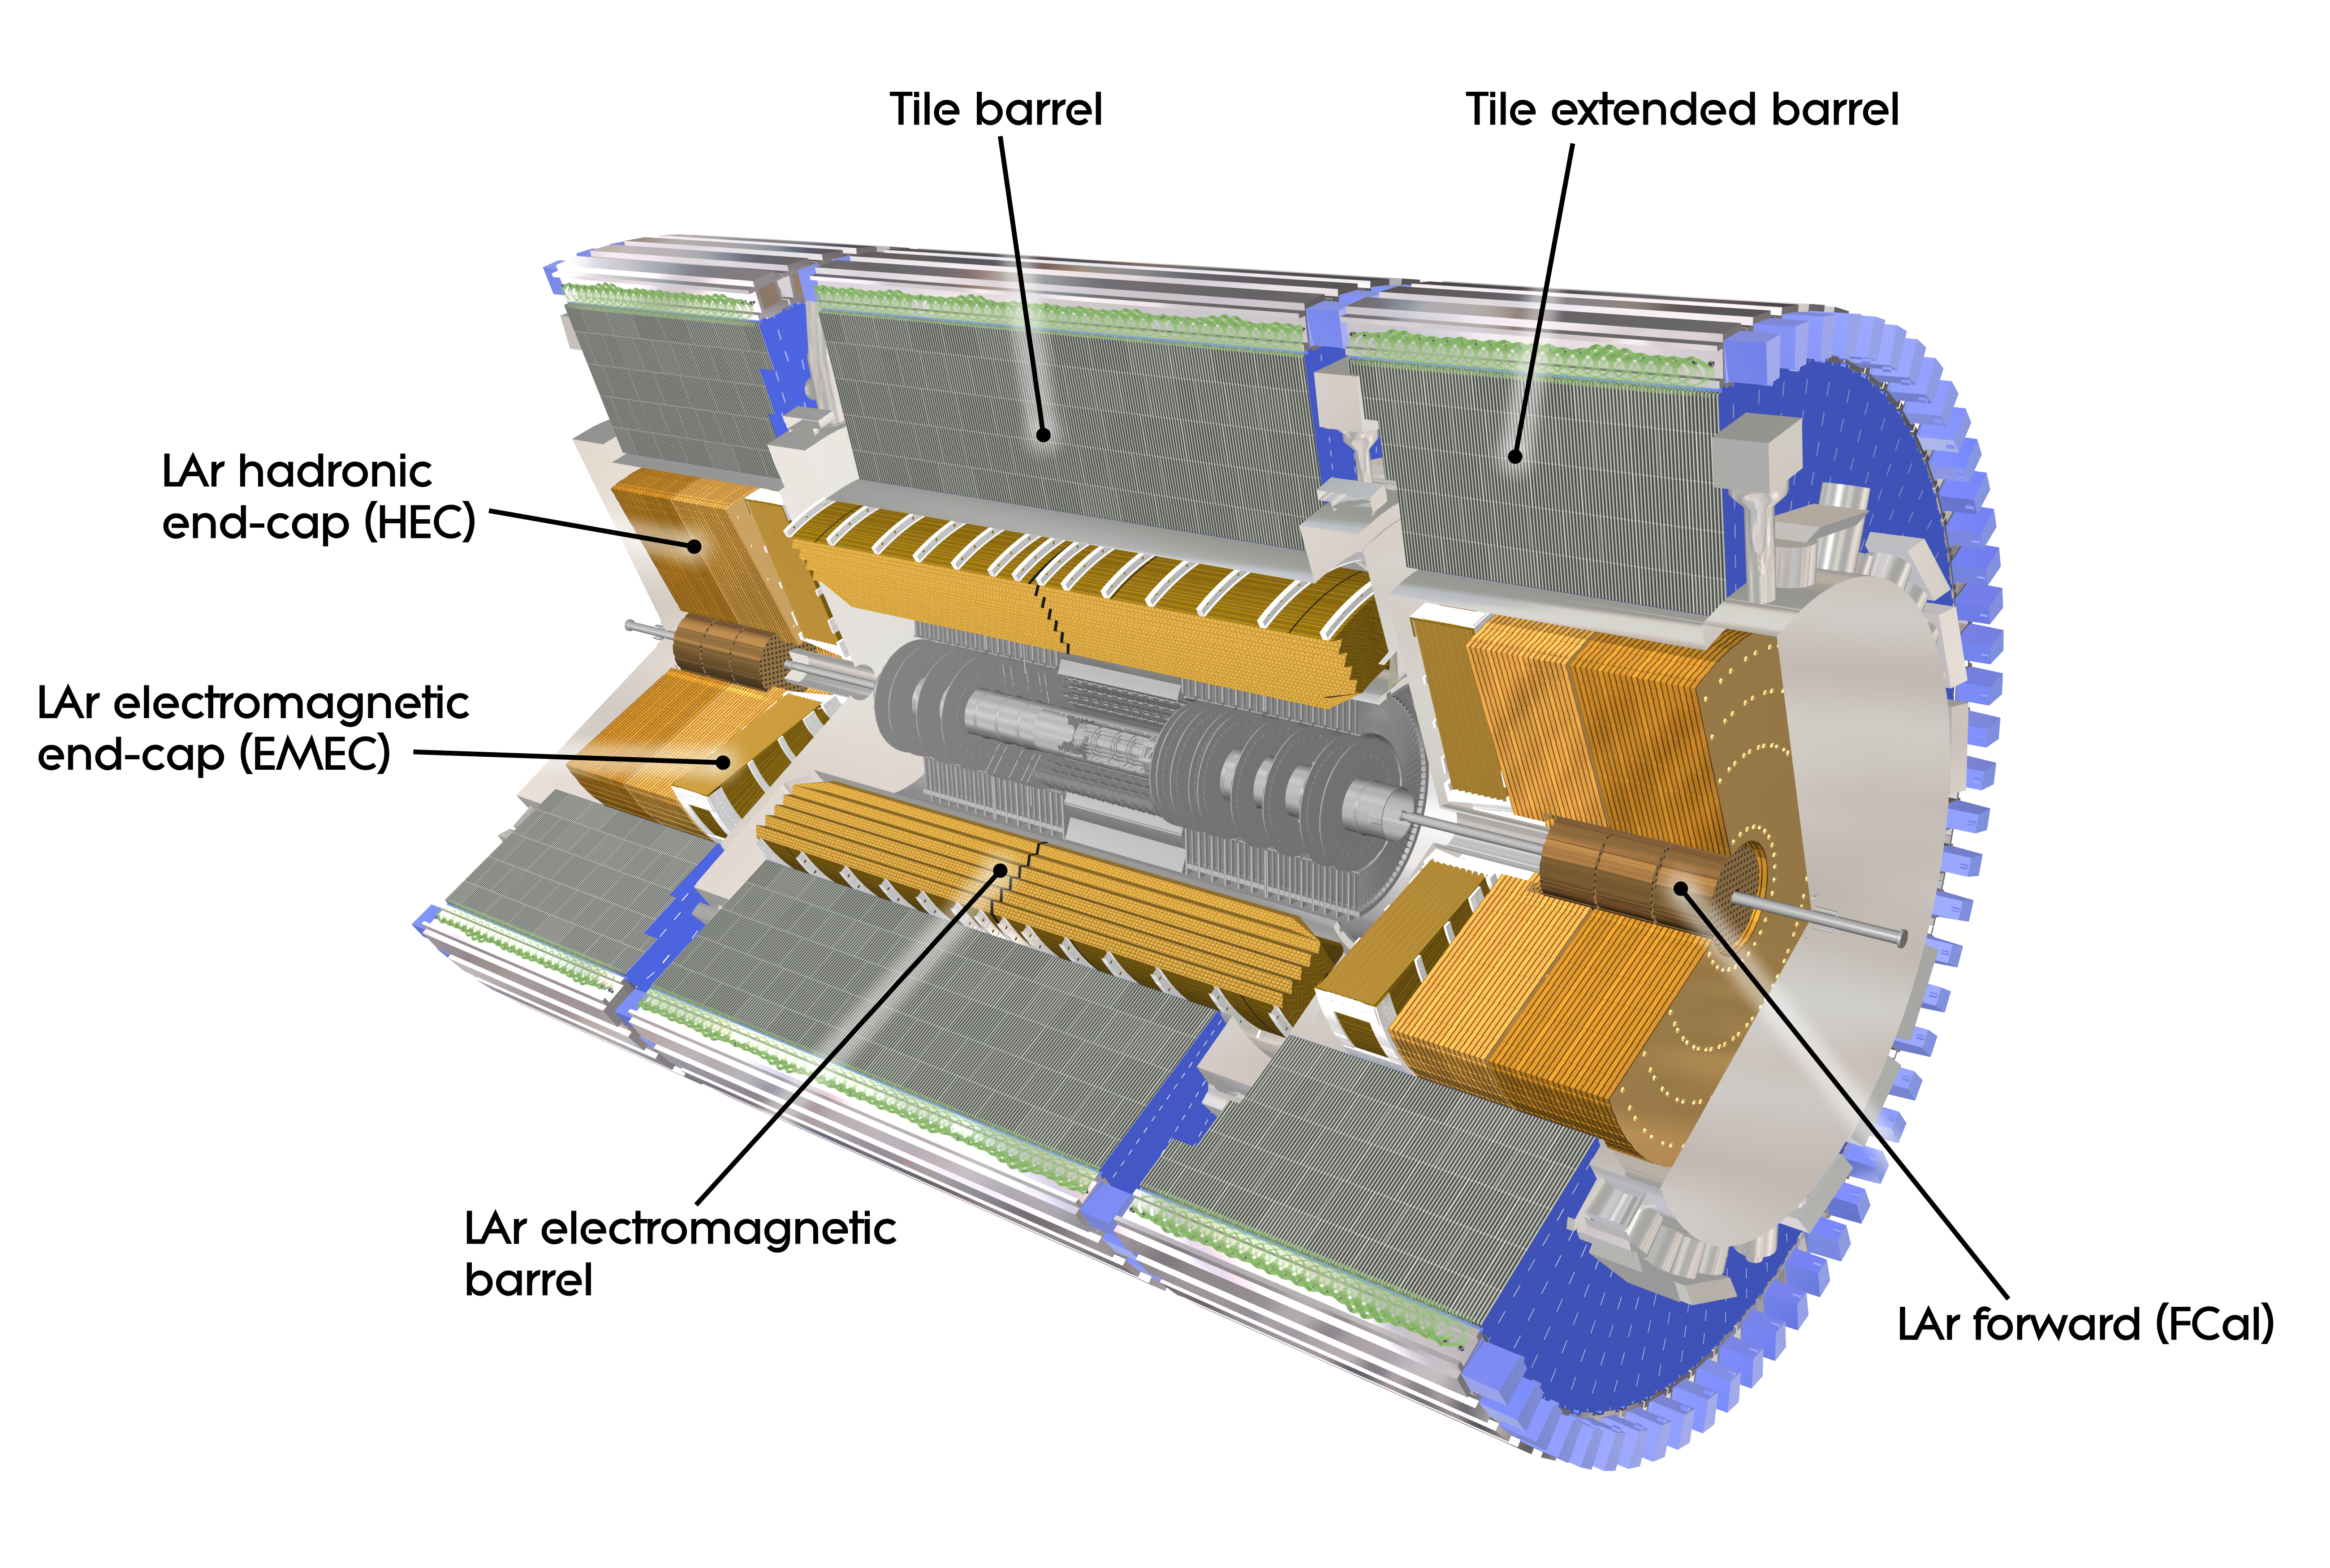
\includegraphics[width=0.75\textwidth]{calorimeters}
	\caption{The ATLAS calorimeter system. The Inner Detector (visible, but greyed out) is enclosed by the Calorimeter system. © 2014 CERN.}
	\label{fig:calorimeter}
\end{figure}

\subsubsection{Electomagnetic Calorimeters}
The Electromagnetic (EM) calorimeter is the innermost layer of the calorimeter system and used for measuring the energy of electrons and photons.
It consists of a high-granularity lead-liquid argon (LAr) electromagnetic (EM) sampling calorimeter which covers the $|\eta| < 3.2$ region.
The energy deposits in the EM calorimeter primarily result from the charged particles in jets, bremsstrahlung radiation produced by electrons, and pair-produced electrons resulting from photons interactions within the calorimeter material.

The EM calorimeter is divided into a Barrel part (EMB) covering $|\eta| < 1.475$ and two End-Caps (EMEC) covering $1.375 < |\eta|\ < 3.2$.
Three separate cryostats are installed to to keep the liquid argon below its boiling point, and the services that compose the End-Cap cryostat necessitate a loss of EM calorimeter coverage in the $1.37 < |\eta|\ < 1.52$ region.
The EMB has three layers, each with slightly different purpose and segmentation granularity, as shown in Fig.~\ref{fig:em_calo_segment}.
The first layer is composed of narrow (in $\eta$) strips which provide precise measurements during the initial showering process.
The second layer is composed of square cells and is designed to fully capture moderate energy $(E < 50 \ \mathrm{GeV})$ photons and electrons.
The final layer of the EMB is less granular and meant to provide additional stopping power for higher energy photons and electrons.
The EMEC follows the EMB segmentation design up until the end of tracking acceptance $(|\eta| < 2.5)$, after which it becomes coarser-grained with only two sampling layers.
\znote{define X0}

\begin{figure}
	\centering
	\includegraphics[width=0.75\textwidth]{em_calo_segment}
	\caption{Sketch of the ATLAS EM barrel calorimeter segmentation around $|\eta| = 0$. 
	The $X_0$ quantity is known as the \textit{radiation length} and quantifies the rate of energy loss with respect to traversed distance as a particle passes through a specific material.
	ATLAS Experiment © 2018 CERN.}
	\label{fig:em_calo_segment}
\end{figure}

\subsubsection{Hadronic Calorimeters}
The hadronic calorimeters are composed of two different technologies in different $|\eta|$ regions of the detector.
In the barrel region $(|\eta| < 1.7)$ resides the Tile Calorimeter composed of alternating layers of plastic active scintillator tiles and steel absorbing tiles.
Like the EM calorimeter, particle showers are induced by the absorbing layer and and particle showers are produced.
Unlike the EM calorimeter, strong force interactions play a role in addition to the electromagnetic interactions, resulting in the presence of hadrons in the showers.
When these hadrons pass through the plastic scintillator material, photons are emitted and detected by photomultipler tubes (PMTs) in order to produce the electrical signals which are then recorded and converted to an energy measurement.
The tiler calorimeter is composed of three sections: one central barrel section $(|\eta| < 1.0)$ and two extended barrels sections $(0.8 < |\eta| < 1.7)$.

The Hadronic End-Cap (HEC) calorimeter provides hadronic energy measurements in the forward $(1.5 < |\eta| < 3.2)$ region.
Like the EM calorimeter it uses liquid argon as the active material, but copper plates as the absorbing layer.
Each wheel of the HEC system is composed of two longitudinal layers, both located directly behind the end-cap cryostats.
\znote{for each calorimeter section, add granularity and dimensions from Tim Bristow thesis}

\subsubsection{Forward Calorimeter}
The forward region $(3.1 < |\eta|\ < 4.9)$ is covered by the Forward Calorimeter (FCal) which measures both electromagnetic and hadronic energy.
The FCal is composed of three concentric cylindrical modules which are themselves composed of a series of rods and tubes, where liquid argon fills the gaps between the rod and tubes as the active medium.
The first modules (closest to the beam line) uses copper as an absorber and performs the electromagnetic energy measurement, while the second and third modules use tungsten as the absorber and perform the hadronic energy measurement.

\subsubsection{Calorimeter Resolution}
The calorimeter energy resolution can be generically parameterized as
\begin{equation}
    \frac{\sigma(E_0)}{E_0} = \frac{a}{\sqrt{E_0}} \oplus \frac{b}{E_0} \oplus c
    \label{eqn:calo_res}
\end{equation}
where $a$ is a stocastic/sampling term representing an intrinsic resolution limit due to particle fluctuations within the shower, $b$ is a noise term determined primarily by electronics noise and pileup, and $c$ is a constant term which dominates at high incident particle energy which is due to non-linearities in calorimeter response caused by inhomogeneity in detector materials, leakage due to un-absorbed particles from the shower, and calibration imperfections.
Each of these quantities $a$, $b$, and $c$ depend on the specific calorimeter detector technology under consideration.
The $\oplus$ operator denotes that each contributing term is summed in quadrature to estimate the final resolution.

The $a$ and $c$ quantities have been carefully measured for the ATLAS calorimeters \cite{Aharrouche_2006} \cite{Strizenec:2009zz} \cite{Cojocaru:2004jk} \cite{Adragna:2009zz} and are summarized in Table~\ref{tab:calo_res}.
The degradation of performance when moving towards higher values of $|\eta|$ is due primarily to the increased presence of pileup in these more forward regions closer to the beam line.
\znote{make sure pileup is defined somewhere previously}
The electronics/pileup noise for each type of calorimeter is shown in Fig.~\ref{fig:calo_noise}.
Increased noise is acceptable in the more forward regions because the higher (on average) incident particle energy there diminishes the effect of the first two terms in Eq. \ref{eqn:calo_res}.

\begin{table}
\centering
\begin{tabular}{|c|c|c|} 
\hline
Region & $a\ [\%]$ & $c\ [\%]$ \\
\hline\hline
EM Barrel & 10.1 $\pm$ 0.1 & 0.17 $\pm$ 0.04 \\
\hline
EM End-Cap & 13.5 $\pm$ 0.5 & 0.7 $\pm$ 0.1 \\
\hline
EM Forward & 29.3 $\pm$ 0.7 & 3.0 $\pm$ 0.1 \\
\hline
Hadronic Barrel & 52.9 $\pm$ 0.9 & 5.7 $\pm$ 0.2 \\
\hline
Hadronic End-Cap & 88.0 $\pm$ 5.0 & 6.8 $\pm$ 0.4 \\
\hline
Hadronic Forward & 98.5 $\pm$ 4.0 & 6.4 $\pm$ 0.04 \\
\hline
\end{tabular}
\caption{
    Measured test beam resolution parameters for the ATLAS calorimeters.
    Each measurement is performed at specific impact points for each separate region: $0 < |\eta| < 0.7$ for the Barrel, $|\eta| = 2.8$ for the End-Caps and $|\eta| = 3.65$ for the Forward region.
}
\label{tab:calo_res}
\end{table}

\begin{figure}
	\centering
	\includegraphics[width=0.75\textwidth]{calo_electronics_noise}
	\caption{Total electronics/pileup noise vs. $|\eta$| at the electron scale, measured in data with 25ns bunch spacing and $\langle \mu \rangle = 14$. ATLAS Experiment © 2015 CERN.}
	\label{fig:calo_noise}
\end{figure}

\subsection{Muon Spectrometer}
\label{sec:muon_spectrometer}
Muons are unique among the common Standard Model $p$-$p$ collision products by virtue of their long lifetime $(2.2 \mu s)$, weakly interacting nature, high production momentum and high mass $(\approx 200 \times m_e)$.
Due to these properties, muons pass through the ATLAS calorimeters without depositing a significant portion of their energy and leave only a weak ionization trail behind.
This necessitates the existence of the final outermost layer of the ATLAS detector: the Muon Spectrometer (MS) \cite{CERN-LHCC-97-022}.

The MS consists of three air-core superconducting toroidal magnet systems (see Fig.~\ref{fig:ATLAS_magnet_system}) and four separate types of tracking chambers covering a region of up to $|\eta| < 2.7$, extending from a radius of 4.25m to 11m.
The magnet system of the MS serves to bend the trajectories of muons in the $R-z$ plane.
The large barrel toroid magnet (0.5 T) is active for $|\eta| < 1.4$, and the two smaller end-cap magnets (1 T) are active in the range $1.6 < |\eta|\ < 2.7$.

\begin{figure}
	\centering
	\includegraphics[width=0.6\textwidth]{magnet_systems}
	\caption{Illustration of the ATLAS magnet system. \cite{CERN-LHCC-97-018}
	The barrel region toroid magnet is shown in red and the two end-cap toroid magnets are shown in green. The inner solenoid is shown in blue, which is parallel to the beam pipe.}
	\label{fig:ATLAS_magnet_system}
\end{figure}

The MS is composed of several different types of detector technologies which are designed for two separate use-cases: (1) extending the precision tracking of each individual muon beyond the ID measurements and (2) fast readouts for the ATLAS trigger system.
Monitored Drift Tube Chambers (MDT) and Cathode Strip Chambers (CSC) are used for the high precision tracking measurements, while Resistive Plate Chambers (RPC) and Thin Gap Chambers (TGC) are less precise but provide a much faster readout, on the scale of nanoseconds, for the trigger system.
The tracking coverage $(|\eta| < 2.7$) of the MS is more complete than the trigger coverage $(|\eta| < 2.4)$.
Like the other major ATLAS detector components, the MS is split into separate barrel $(|\eta| < 1.05)$ and endcap $(|\eta| < 2.7)$ regions.

\begin{figure}
	\centering
	\includegraphics[width=0.75\textwidth]{muon_subsystem}
	\caption{ATLAS Experiment © 2014 CERN}
\end{figure}

The MDT chambers are used for precision tracking of the $R-z$ plane curvature of muons.
They consist of 3-8 layers of 30mm diameter drift tubes between 0.8m and 6.5m long, filled with a mixture of $Ar/CO_2$ gas held at a pressure of three atmospheres.
Whenever the gas inside the drift tube is ionized by a passing muon, the resulting free electrons drift towards a 50 $\mu m$ W-Rh anode wire held at a voltage of 3kV in the center of the tube.
The precision tracking data from the barrel is measured by MDT chambers that cover the $|\eta| < 2$ range in the first layer, and up to $|\eta| < 2.7$ in the two outer layers.
There are three concentric barrel layers composed of MDT and RPC chambers at radii of 5m, 7.5m, and 10m.

The RPC chambers measure the non-bending coordinate ($\phi$) of muons.
They are composed of a set of parallel plate capacitors separated by a 2mm insulating space filled with a gas mixture of predominantly tetrafluoroethane ($C_2 H_2 F_4$). 
The plates have high resistance and are held at a constant high voltage, with metallic strips attached to their outer faces.
The fast response time of the RPC technology (1.5ns) makes it a prime candidate for the muon trigger system.
The RPC chambers are attached to the MDT chambers in the barrel and cover the central $|\eta| < 1.05$ region.

The CSC chambers replace the MDTs in the forward region of the first barrel layer of the MS in order to account for the high interaction rate in this region that would otherwise cause significantly degraded performance of the MDTs in this region ($2 < |\eta| < 2.7)$).
The CSC detector region is organized into two disks of sixteen chambers each.
Each CSC chamber consists of both a multi-wire proportional drift chamber as well as interleaved cathode strips placed parallel and perpendicular to the anode multi-wire layers.
The parallel cathode strips provide precision tracking measurement in the bending plane, while the perpendicular cathode strips provide measured of $\phi$.

The TGC chambers are similar to the CSC chambers in design and consist of 50 $\mu m$ gold-plated tungsten anode wires, but with smaller gaps between electrodes for faster readouts.
They only provide measurement of the $\phi$ coordinate and cover the $1.0 < |\eta| < 2.4$ region.

\begin{figure}
	\centering
	\includegraphics[width=0.9\textwidth]{muon_spectrometer_quadrant}
	\caption{
	 Cross-section of a quadrant of the ATLAS Muon Spectrometer \cite{kuger2017signal} in the $R-z$ plane (left) and the $R-\phi$ plane (right) comprising all detector modules. The naming of MDT chambers is based on their location in the barrel or end-cap (B,E), in the inner, middle, or outer layer (I, M, O) and in either the a large or a small sector (L,S).
	}
\end{figure}

% \subsection{Forward Detectors}
% The ATLAS experiment has additional detectors situated far away (20+ meters) from the interaction point which each serve a unique, specialized purpose.
% 
\subsection{Trigger and DAQ}
The LHC currently operates at a collision rate of 40 MHz.
Given that each event requires approximately 1.5 MB of disk storage, it is impractical to attempt to record every collision event observed by the ATLAS detector.
Not only would this would require a bandwidth of $> 60$ TB/s, but most events are not of any serious interest to HEP research efforts.
For this reason the ATLAS trigger system \cite{Ruiz-Martinez:2133909} is used to reduce the recorded event rate to a more manageable level of approximately 1-2 KHz, which reduces the bandwidth requirement to GB/s or less.
The trigger system operates in real-time at both hardware and software levels and ensures only events of interest to ongoing research are recorded by the ATLAS data acquisition system (DAQ).
For Run-2 ATLAS uses a two-tier trigger system: a hardware-based ``level-1'' (L1) trigger followed by a software based ``high-level'' (HLT) trigger.
Each trigger in the chain significantly reduces the data rate.
Only the events selected by the HLT are actually stored for offline processing/analysis.
A schematic of the full ATLAS trigger/DAQ system is shown in Fig.~\ref{fig:trigger_system}.

\begin{figure}
	\centering
	\includegraphics[width=0.8\textwidth]{atlas_trigger_system}
	\caption{Schematic layout of the ATLAS trigger and data scquisition system for Run-2. \cite{Ruiz-Martinez:2133909}}
	\label{fig:trigger_system}
\end{figure}

\subsubsection{Level 1 Trigger}
The Level 1 (L1) Trigger is a physical electronic device located within the ATLAS detector which has sub-components that communicate with hardware from both the calorimeter (L1Calo) and muon spectrometer (L1Muon).
The L1Muon trigger processor interfaces directly with the dedicated muon trigger chamber hardware described in Section~\ref{sec:muon_spectrometer}.
The L1Calo trigger processor, on the other hand, relies on a form of modified calorimeter output called \textit{calorimeter trigger towers}.
These trigger towers consist of energy and timing sums for calorimeter regions with reduced granularity ($\Delta \eta \times \Delta \phi)$ ranging from $0.1 \times 0.1$ in the central region to $0.4 \times 0.4$ in the forward region.
A newer hardware-based L1 trigger labeled L1Topo actually analyzes kinematic/geometric relationships between different objects.
\znote{expand section about L1Topo}

The Central Trigger Processor (CTP) receives all the information in real-time from the L1Muon, L1Calo, and L1Topo processors.
The CTP first synchronizes the trigger inputs with the LHC collision clock in order to correctly associate each event with the correct bunch crossing.
All trigger inputs are then compared to different sets of trigger thresholds defined for each separate type of physics beind targeted by ATLAS.
The choice of trigger thresholds are ultimately determined by the maximum allowed L1 output rate of 100 KHz, which represents a factor of 400 reduction from the 40 MHz event rate at the LHC.
If any set of trigger thresholds are passed, the CTP flags the event as accepted and notifies all sub-detectors.
Upon receiving this ``L1 Accept'' (L1A) notification, all the data from each sub-detector is read out and propagated to the next step in the trigger process: the High Level Trigger.
\znote{mention ROIs}

\subsubsection{High Level Trigger}
The HLT is a software based trigger that refines set of events passing the L1 trigger using the full information available from the ATLAS detector, as opposed to the low granularity data used by the L1 trigger.
For example, the HLT uses tracking information from the ID to locate the primary vertex (PV) \znote{cite vertexing section} and various particle candidates.
The HLT reduces the data rate from 100 KHz to approximately 1 KHz.
Since the HLT is software based it is limited primarily by the CPU processing time and must be highly optimized to process each event in approximately 0.1 - 1.0 seconds.
An example of such an optimization is that track reconstruction \znote{cite tracking section} is only performed within ROIs identified by the L1 trigger.

\subsection{Computing}
The raw data for all events passing the ATLAS trigger system is sent to CERN Data Center where the process of archiving, distributing, processing and analyzing begins.
However, this is only the starting point of an international network of LHC computing resources \cite{Bird:1447125} known as the Worldwide LHC Computing Grid (WLCG) or simply ``the grid''.
The WLCG is a layered system made up of four separate ``tiers'' as shown in Fig.~\ref{fig:wlcg_tiers}.

\begin{figure}
	\centering
	\includegraphics[width=0.65\textwidth]{wlcg_tiers}
	\caption{Schematic diagram of the Worldwide LHC Computing Grid (WLCG) tier system. © 2020 CERN.}
	\label{fig:wlcg_tiers}
\end{figure}

The CERN Data Center (\textbf{Tier-0}) provides around 20\% of the total compute capacity of the LHC, with the other 80\% coming from institutions around the world.
The next layer of support (\textbf{Tier-1}) is composed of thirteen large computing centers with round-the-clock support and massive storage capacity.
They are responsible for large-scale reprocessing, storage and safe-keeping of a significant proportion of raw and reconstructed data from the LHC.
Furthermore, Tier-1 centers share these resources with the next link in the chain (Tier-2).
Tier-1 centers are typically national laboratories such as BNL, INFN, and TRIUMF.

The next link in the chain (\textbf{Tier-2}) is composed primarily of universities and other scientific institutions which posses enough storage and computing power for a combination of analysis tasks, simulated event production and reconstruction.
Individual scientists connect to the grid via the last tier (\textbf{Tier-3}) which consists of local computing resources such as small local clusters belonging to individual Physics departments or event individual PCs.

\graphicspath{{Ch3_Reconstruction/figures/}}

\chapter{ATLAS Object Reconstruction and Particle Identification}

% TODO: define different particle types/families in Theory section and refer to here
A large number of particles are produced during a $p$-$p$ collision event.
These include charged particles such as electrons $(e^\pm)$, muons $(\mu^\pm)$ and charged hadrons $(\pi^\pm)$ as well as electrically neutral particles such as photons $(\gamma)$, neutrinos $(\nu_e, \nu_\mu, \nu_\tau)$ and and neutral hadrons $(\pi^0)$.
In order to achieve the wide range of physics goals of the ATLAS experiment, all of these particles must be reconstructed and identified with high efficiency.
Furthermore, the properties of these objects must be measured with a high degree of precision and accuracy.
This requires maximal utilization of the output from all ATLAS subdetectors.

% plot: number of interaction vertices
% plot: number of charged particles (or tracks) per event
% plot: event display

\section{Tracks}
\label{sec:tracking}
The reconstruction of charged particle trajectories within the ATLAS detector is important for nearly all physics object identification and reconstruction.
These reconstructed trajectories are referred to as \textit{tracks} and the procedure for identifying and reconstructing all the charged particle trajectories in each event is called \textit{tracking}.
Tracking begins with the measurement of the particles position at multiple points within the ID (Section~\ref{sec:inner_detector}) each referred to as a \textit{hit}.

The tracking procedure for ATLAS is divided into four separate stages \cite{Salzburger:2015sgq}:

\begin{enumerate}
    \item \textbf{Data Preparation and Space Point Formation}\\
        When a charged particle passes thorugh the active silicon material of the various ID sub-detectors, it leaves behind \textit{clusters} of 
        raw data output spanning multiple nearby sensors of the various ID sub-detectors.
        The first tracking stage consists of finding these connected clusters and associating them together into a single three-dimensional location.
        This difficulty of this process is compounded by the fact that nearby particle trajectories in dense environments can often \textit{merge} together into the same cluster.
        This necessitates the use of a neural network based cluster splitting routine for the Pixel detector.
        After clusters are identified and (potentially) split, their locations are transformed from the local subdetector cooordinate system to the global ATLAS coordinate system and referred to as \textit{space points}.
    \item \textbf{Space Point Seeded Track Finding}\\
        The process of converting space points into actual tracks begins by forming track \textit{seeds} built from triplets of space points.
        These triplets may come from any combination of space points from either of two innermost ID sub-detectors: Pixel and SCT.
        To reduce the number of potential seeds, each individual space point is restricted to appear in only a small number of seeds.
        Seeds which pass a set of loose initial requirements are passed to a \textit{track finding algorithm} which utilizes the Kalman Filter technique.
        The goal at this stage is to produce a set of \textit{track candidates}, consisting only of space points within the Pixel/SCT detectors, to pass forward to the next tracking stages.
    \item \textbf{Ambiguity Solving}\\
        At this stage, some of the track candidates may be \textit{fake} or \textit{duplicates}.
        Fake tracks result from a random combination of space points that manage to pass the loose quality requirements of the track seeding described above.
        Because space points are allowed to be shared between different track candidates, it is also for the same charged particle to manifest as two separate track candidates.
        At this stage it is necessary to reject as many of these fake/duplicate tracks as possible.
        The \textit{ambiguity solving algorithm} achieves this by scoring track candidates.
        Positive scores are gained by track candidates that possess unique (non-shared) space points and good fit quality from the Kalman Filter algorithm.
        Negative scores are assigned to track candidates which possess shared hits or missing hits (called \textit{holes}) in a Pixel/SCT layer where they would be expected.
    \item \textbf{TRT Extension}\\
        After passing the ambiguity resolution stage, the final set of track candidates are extended to include hits from the TRT, the outermost ID sub-detector.
        This process is only performed for track candidates within the acceptance of the TRT.
        When the TRT extension is successful, the momentum resolution is significantly improved.
\end{enumerate}

This resulting tracks are then individually fit with a $\chi^2$ minimization routine \cite{Cornelissen:2008zza} which accounts for the magnetic field strength in each region of the detector. This final track fitting produces an estimate of the \textit{track parameters}.

The track selection requirements are
\begin{enumerate}
    \itemsep0em 
    \item \textbf{Loose} \begin{itemize}
        \itemsep0em 
        \item $p_T > 400$\ MeV
        \item $|\eta| < 2.5$
        \item number of silicon (IBL + Pixel + SCT) hits $\geq$ 7
        \item number of shared modules $\leq 1$
        \item number of silicon holes $\leq 2$
        \item number of pixel holes $\leq 1$
    \end{itemize}
    
    \item \textbf{Tight} \footnote{The Tight selection requirements are applied \textit{on top of} the Loose requirements.} \begin{itemize}
        \itemsep0em 
        \item if $|\eta| \leq 1.65$, number of silicon hits $\geq 9$
        \item if $|\eta| > 1.65$, number of silicon hits $\geq 11$
        \item either one IBL or next-to-innermost-Pixel-layer hit
        \item no Pixel holes
    \end{itemize}
\end{enumerate}

\begin{figure}
	\centering
	\includegraphics[width=\textwidth]{id_subdetector_hits}
	\caption{Comparison of the number of (a) IBL, (b) Pixel, (c) SCT, and (d) TRT tracking hits distributions in data and simulation for the Loose track selection. The distributions are normalized to one so that the bin contents represent track fraction. \cite{ATL-PHYS-PUB-2015-018}
	}
	\label{fig:id_subdetector_hits}
\end{figure}

\section{Vertex}
In order to perform physics analysis it is vital to determine the location of the individual proton-proton collisions in each event at the ATLAS detector.
% TODO: define track parameters, impact parameters in tracking section
The \textit{vertex finding} algorithm is divided into four major steps which are iterated numerous times to reconstruct each vertex in the event  \cite{Borissov:2015djv}:
\begin{enumerate}
    \item 
        The arithmetic mode of the $z_0$ impact parameter for all (remaining) tracks in an event is computed in order to produce an initial \textit{seed} vertex.
    \item 
        Tracks compatible with the seed are grouped together for fitting.
    \item 
        The adaptive vertex fitting algorithm is used to estimate the position and uncertainty of the vertex.
    \item
        Remaining tracks that are incompatible with this new vertex are removed and used to repeat the entire procedure again, starting by computing a new seed.
\end{enumerate}
This vertex finding algorithm is tuned to balance two competing difficulties: (1) Splitting a real vertex into multiple reconstructed vertices and (2) merging two proton-proton interactions into the same reconstruction vertex. 
The vertex with the largest $\sum p_T^2$ for all associated tracks is termed the hard-scatter vertex. In general all physics analysis work considers only objects associated to this vertex, while all other reconstructed vertices are considered to be the result of pile-up.

\section{Electrons}
Electrons interact primarily with the EM calorimeters (described in ~\ref{sec:calorimeters}) by leaving a signature in groups of neighboring cells.
The reconstruction of electrons is performed by matching reconstructed tracks from the ID with these calorimeter deposits.
Electron reconstruction in the central region of the ATLAS detector ($|\eta| < 2.47$) proceeds in several steps \cite{ATLAS-CONF-2016-024}:

\begin{enumerate}
    \item \textbf{Seed-Cluster Reconstruction}\\
        A $3 \times 5$ sliding window\footnote{The sliding window grid has has units of $0.025 \times 0.025$ in $(\eta, \phi)$ space, which corresponds to the granularity of the middle layer of the EM calorimeter.} is used to search for electron cluster \textit{seeds}.
        For position of the sliding window the total energy is summed across all longitudinal layers for each contained cell, forming a so-called \textit{tower}.
        If the sum of transverse energy from the towers in the window is greater than 2.5 GeV, a seed cluster is formed.
        If the seed cluster passes certain quality requirements a \textit{Region of Interest} (ROI) is specified surrounding the location of the cluster.
    \item \textbf{Track Reconstruction}\\
        Several intricacies of the track-fitting (described in Section \ref{sec:tracking}) are modified in order to assist with the reconstruction of electrons.
        By default the ATLAS tracking procedure assumes tracks correspond to particles with an energy loss model corresponding to pions.
        However, this model can be substituted for an alternative model allows for up to 30\% energy loss at each intersection of the track with the ID material.
        This alternative model accounts for the possibility of bremsstrahlung.
        During the execution of the tracking algorithm, if a track seed with $p_T > 1$ GeV can not be extended into a full track with at least seven hits using the pion energy loss model, a second attempt is performed using the electron energy loss hypothesis.
        Furhermore, if a track candidate is produced with the pion hypotehsis but fails the final Global $\chi^2$ track fit, it is then refit with the electron hypothesis.
        Tracks utilizing the electron hypothesis are tagged as such and utilized in the next steps of the electron reconstruction process.
    \item \textbf{Electron-Specific Track Fit}\\
        The tracks obtained in the previous step are then loosely matched to the EM clusters based on their separation in the $\eta-\phi$ plane.
        In order to perform this matching the trajectory of the track is extended into the center of the EM calorimeter.
        Tracks with $\geq 4$ precision hits and are loosely associated to electron clusters are refit using an optimized Gaussian Sum Filter (GSF) \cite{ATLAS-CONF-2012-047} which is specialized to account for non-linear bremsstrahlung effects.
        A similar but stricter matching as the one described above is performed again with the refitted track.
    \item \textbf{Electron Candidate Reconstruction}\\
        If multiple tracks fulfill the matching criteria for the same EM cluster, one of them is chosen as the \textit{primary} track.
        The choice is based upon a number of criteria: (1) cluster-track distance in the $\eta-\phi$ plane, (2) number of hits in the Pixel detector and (3) the presence of a hit in the first silicon layer.
        If a cluster is not associated to any tracks at this point, it is removed and considered as a photon candidate.
        The efficiency of electron idenficiation is shown in Figure~\ref{fig:electron_eff_Zee}.
        The energy of the clusters is then calibrated to match that of the original electron energy using multivariate techniques based on simulated MC samples \cite{Aaboud:2018ugz}.
        The four-momentum of the electron is then computing using the energy information from the final calibrated energy of the cluster and directional information ($\eta, \phi$) from the best track matched to the original seed cluster.
\end{enumerate}

\begin{figure}
	\centering
	\includegraphics[width=0.65\textwidth]{electron_eff_Zee}
	\caption{
	    The electron identification efficiency in $Z \rightarrow ee$ events in data as a function of transverse energy ($E_T$) for the Loose, Medium, and Tight working points.
	    The efficiency in data is obtained by applying data-to-simulation efficiency ratios that are measured in $J/\psi \rightarrow ee$ and $Z \rightarrow ee$ events to the $Z \rightarrow ee$ simulation.
	    \cite{Aaboud:2018ugz}
	}
	\label{fig:electron_eff_Zee}
\end{figure}

\section{Muons}
Muons are a minimum ionizing particle and interact weakly with the ATLAS calorimeter system, depositing approximately 3-4 GeV there on average \cite{Lenzi_2010}.
Thus, as discussed in Section \ref{sec:muon_spectrometer}, muons are reconstructed primarily by combining tracking information from the ID and MS.
Within the ID, tracks from muons are not treated any differently than any other type of charged particle.
Within each sub-detector region of the MS (MDTs, CSCs, etc) a Hough transform \cite{10.1016/S0734-189X(88)80033-1} is used to search for hits aligned in the bending plane of the detector (produced by the magnetic field) and produce muon \textit{track candidates}.
Track candidates are formed by combining hits from different track segments via a combinatorial search \cite{Aad:2016jkr}.
After this an overlap removal algorithm is run to find the most optimal track assignment.
The final track candidates are fit with a global $\chi^2$ minimiazation algorithm, similar to ID track reconstruction.
Finally, a hit recovery and track re-fit are performed if necessary.

Four types of muons emerge from the reconstruction process, depending on which sub-detectors are involved:
\begin{itemize}
    \item \textbf{Combined Muons (CB)}\\
        A global fit is used to combine hits form both the ID and the MS.
        The track from the MS is used as the primary starting point and extrapolated inward and matched to a single ID track.
        These are the most common types of reconstructed muons used in physics analyses, as they have the highest purity and best kinematic resolution.
    \item \textbf{Segment-Tagged Muons (ST)}\\
        Like the CB muons, ST muons are constructed by combining ID and MS hits.
        However, in the case of ST muons, a local track segment from either the MDT or CSC chambers is used in place of a full MS track.
        This strategy is necessary for reconstructing muons which cross only one layer of the MS chambers.
        This typically occurs when the muon possesses low $p_T$ and passes through only one region of the MS.
    \item \textbf{Calorimeter-Tagged Muons (CT)}\\
        In the case where an ID track can be matched to a deposit in the calorimeter system which is compatible with a minimum ionizing particle, some muons can be reconstructed in regions where the MS has low acceptance around $|\eta| \approx 0$.
    \item \textbf{Extrapolated Muons (ME)}\\
        In the region beyond the ID acceptance but still within the MS acceptance ($2.5 < |\eta| < 2.7$) some muons can still be reconstructed by utilizing only MS tracks. A loose requirement is placed to ensure the MS track pointers towards the IP.
\end{itemize}

As with electrons, muon candidates can be categorized according to purity: ``Loose'', ``Medium'', and ``Tight''.
The muon reconstruction efficiency at ATLAS is nearly 100\%, as seen in Figures TODO.

%TODO: discuss electron/muon isolation.

\section{Event Data Model}
% \cite{Buckley:2014150}
The design of data structures for representing a collider event, the Event Data Model (EDM), has significant ramifications for both computing efficiency as well as the overall productivity of the scientists analyzing the output of the ATLAS detector.
The analysis described in this thesis, like most ATLAS research efforts, follows trajectory of gradually simpler data formats: 
% \begin{align}
% xAOD $\rightarrow$ DxAOD $\rightarrow$ CxAOD $\rightarrow$ $n$-tuple $\rightarrow$ histogram.
% \end{align}

\subsubsection{RAW (DATA)}
\subsubsection{EVNT (MC)}
\subsubsection{HITS (MC)}
\subsubsection{RDO (MC)}
\subsubsection{xAOD}
\subsubsection{DxAOD}
\subsubsection{CxAOD}
\subsubsection{$n$-tuple}


\graphicspath{{Ch4_Jets/figures/}}

\chapter{Jets}
\dots
\section{Jet Reconstruction}
\dots
\subsection{Jet Clustering}
\dots
\subsection{Large-Radius Jets}
\dots
\subsection{Track Jets}
\dots
\section{Jet Calibration}
\dots
\section{Jet Substructure}
\dots
\section{B-Jet Identification}
\dots
\graphicspath{{Ch5_VHqqbb/figures/}}

\chapter{All-Hadronic VH Resonance Search}

This thesis presents the ATLAS search for new resonances decaying to a vector boson $V = W,Z$ and a Standard Model (SM) Higgs boson $H$, in the fully hadronic $q\bar{q}^{(\prime)}b\bar{b}$ decay channels.
This search focuses on new resonance masses of $m_{VH} \geq 1.5$~TeV.
The $V$ and $H$ bosons that are produced in the decay of such heavy resonances are highly boosted and the resulting decay products of each boson are likely to be collimated and merged into a single large radius jet.
The dijet invariant mass spectrum of the two large radius jets is then used as discriminant variable, where the signature of the new heavy resonance decay yields a resonant structure on top of the smoothly falling background.
The dominant background ($\approx$ 90\%) corresponds to multijet QCD processes, with much smaller contributions from other non-resonant backgrounds: $t\bar{t}$ and $V$ + jets.
After reconstructing the $V$ and $H$ boson candidates as large radius jets, the tools of jet substructure and b-tagging are applied to heavily suppress the dominant background of multijet events.
Due to the challenges associated with modelling this background with Monte Carlo (MC) samples, a fully data-driven method is used to provide a background estimation method.

%TODO: define dijet mass very clearly

A simplified model \cite{Pappadopulo:2014qza} fulfilling only SM symmetry constraints is used to provide a model-independent Lagrangian for a heavy resonance search.
This framework incorporates Heavy Vector Triplets (HVT), a common SM extension with an isospin $SU(2)_{L}$ triplet formed of a neutral $Z'$ and two charged $W^{\prime \pm}$ bosons, from which two explicit models will be considered as benchmarks to evaluate the relative sensitivity of this analysis to $W^{\prime \pm}$ and $Z'$ signals: Models A and B \cite{Pappadopulo:2014qza}, where weakly and strongly coupling scenarios are described, respectively.
The couplings of the new vector bosons $W^{\prime \pm}$, $Z'$ to the $H$ and $V$ bosons are defined as a combination of parameters $g_{V}c_{H}$, while the couplings to fermions are defined as $(g^{2}/g_{V})c_{F}$, where $g_V$ represents the strength of the new vector boson interaction and $c_{H}$ ($c_{F}$) represents the coupling to the Higgs boson (fermions).
In Model A, the branching fractions to fermions and gauge bosons are comparable, whereas in Model B the fermionic couplings are suppressed.

A search for heavy vector resonances decaying to $VH$ in the fully hadronic final state was previously performed in ATLAS using $36.1\pm1.0\text{~fb}^{-1}$ of $pp$ collision data at 13 TeV taken during 2015 and 2016 \cite{Aaboud:2017ahz}.
The largest excess was observed in the $ZH$ channel at $m_{JJ}\sim3.0$~TeV with a local significance of 3.3~$\sigma$, with a  global significance of  2.2~$\sigma$.
Upper limits on the production cross-section times branching ratio to the $q\bar{q}^{(\prime)}b\bar{b}$ final state were set for resonance masses in the range between 1000 and 3800 GeV with values ranging between 107 to 3 fb and 97 to 2 fb (at 95\% CL) for $WH$ and $ZH$ resonances, respectively.
The corresponding excluded HVT Model B signal mass ranges are 1000-2500 GeV for $WH$ resonances, and 1000 - 2600 GeV for $ZH$ resonances.

Searches for heavy vector resonances decaying to $VH$ in the $V$ boson leptonic decay channels have been performed in ATLAS using $36.1\pm1.0\text{~fb}^{-1}$ of $pp$ collision data at 13 TeV \cite{EXOT-2016-10}.
For HVT Model A $W'$ ($Z'$) masses have been excluded up to 2.67 TeV (2.65 TeV), while for Model B, $W'$ ($Z'$) masses of up to 2.86 TeV (2.83 TeV) have been excluded.

The CMS collaboration has published a search for new heavy objects decaying to $VH$ in the fully hadronic mode using $19.7$~fb$^{-1}$ of 8 TeV data from Run 1 of the LHC.
Resonance masses up to 1.7 TeV were excluded in the combined $W'$ and $Z'$ search (1.1 TeV in \zpzh, 1.5 TeV in \wpwh), using the HVT Model B benchmark \cite{Khachatryan:2015bma}.
The search was also performed by CMS using $35.9$~fb$^{-1}$ of 13 TeV data from Run 2 of the LHC, excluding $W'$ ($Z'$) bosons with masses up to 3.15 TeV (2.26 TeV, except 1.19-1.21 TeV) in Model B \cite{Sirunyan:2017wto}.

% TODO: adapt this summary to thesis .tex structure
%This note is structured as follows: Section \ref{sec:samples} describes the data and simulated samples; Section \ref{sec:objects} and \ref{sec:selection} describe the object definitions and event selections and corresponding optimization studies; Section \ref{sec:background} describes the strategy for background estimation; Section \ref{sec:syst} describes the systematic uncertainties considered in this search; finally Sections \ref{sec:result} and \ref{sec:conclusion} present the results and conclusions of this search.

\section{Theoretical Motivation/Overview}
%TODO: describe HVT Model A/B distinction

\begin{figure}
	\centering
	\includegraphics[width=0.75\textwidth,angle=90,origin=c]{feynman_diagram_VHqqbb}
	\caption{
	Feynman diagram illustrating the $pp \rightarrow V^\prime \rightarrow VH$ production/decay chain searched for in this analysis.
	}
	\label{fig:feynman_diagram_VHqqbb}
\end{figure}

\dots

\section{Analysis Strategy}
\dots

\section{Data and Simulated Samples}

Tables~\ref{tab:hvta_wh} and ~\ref{tab:hvta_zh} summarize the properties of the HVT Model A signal samples generated and used for this analysis, while Tables~\ref{tab:hvtb_wh} and ~\ref{tab:hvtb_zh} describe HVT Model B.

\begin{table}[!htb]
\begin{scriptsize}
\begin{center}
\begin{tabular}{|c|l|c|c|c|c|r|}
\hline
DSID & Process & Generator & $\sigma$ [fb] & $k$-factor & $\epsilon_{\text{filter}}$ & Events \\ \hline
302321 & \makecell{HVT $W^{\prime} \rightarrow WH \rightarrow qq^\prime(b\bar{b} + c\bar{c})$ \\ Model A, m = 1000 GeV} & \makecell{\MADGRAPH v2.2.2 + \PYTHIA v8.186 \\ + EvtGen v1.2.0} & 4.334e+02 & 1.0 & 1.0 & 110000 \\
\hline
302322 & \makecell{HVT $W^{\prime} \rightarrow WH \rightarrow qq^\prime(b\bar{b} + c\bar{c})$ \\ Model A, m = 1100 GeV} & \makecell{\MADGRAPH v2.2.2 + \PYTHIA v8.186 \\ + EvtGen v1.2.0} & 2.901e+02 & 1.0 & 1.0 & 110000 \\
\hline
302323 & \makecell{HVT $W^{\prime} \rightarrow WH \rightarrow qq^\prime(b\bar{b} + c\bar{c})$ \\ Model A, m = 1200 GeV} & \makecell{\MADGRAPH v2.2.2 + \PYTHIA v8.186 \\ + EvtGen v1.2.0} & 1.995e+02 & 1.0 & 1.0 & 110000 \\
\hline
302324 & \makecell{HVT $W^{\prime} \rightarrow WH \rightarrow qq^\prime(b\bar{b} + c\bar{c})$ \\ Model A, m = 1300 GeV} & \makecell{\MADGRAPH v2.2.2 + \PYTHIA v8.186 \\ + EvtGen v1.2.0} & 1.401e+02 & 1.0 & 1.0 & 95000 \\
\hline
302325 & \makecell{HVT $W^{\prime} \rightarrow WH \rightarrow qq^\prime(b\bar{b} + c\bar{c})$ \\ Model A, m = 1400 GeV} & \makecell{\MADGRAPH v2.2.2 + \PYTHIA v8.186 \\ + EvtGen v1.2.0} & 1.002e+02 & 1.0 & 1.0 & 125000 \\
\hline
302326 & \makecell{HVT $W^{\prime} \rightarrow WH \rightarrow qq^\prime(b\bar{b} + c\bar{c})$ \\ Model A, m = 1500 GeV} & \makecell{\MADGRAPH v2.2.2 + \PYTHIA v8.186 \\ + EvtGen v1.2.0} & 7.283e+01 & 1.0 & 1.0 & 80000 \\
\hline
302327 & \makecell{HVT $W^{\prime} \rightarrow WH \rightarrow qq^\prime(b\bar{b} + c\bar{c})$ \\ Model A, m = 1600 GeV} & \makecell{\MADGRAPH v2.2.3 + \PYTHIA v8.186 \\ + EvtGen v1.2.0} & 5.367e+01 & 1.0 & 1.0 & 110000 \\
\hline
302328 & \makecell{HVT $W^{\prime} \rightarrow WH \rightarrow qq^\prime(b\bar{b} + c\bar{c})$ \\ Model A, m = 1700 GeV} & \makecell{\MADGRAPH v2.2.2 + \PYTHIA v8.186 \\ + EvtGen v1.2.0} & 3.999e+01 & 1.0 & 1.0 & 110000 \\
\hline
302329 & \makecell{HVT $W^{\prime} \rightarrow WH \rightarrow qq^\prime(b\bar{b} + c\bar{c})$ \\ Model A, m = 1800 GeV} & \makecell{\MADGRAPH v2.2.3 + \PYTHIA v8.186 \\ + EvtGen v1.2.0} & 3.012e+01 & 1.0 & 1.0 & 110000 \\
\hline
302330 & \makecell{HVT $W^{\prime} \rightarrow WH \rightarrow qq^\prime(b\bar{b} + c\bar{c})$ \\ Model A, m = 1900 GeV} & \makecell{\MADGRAPH v2.2.2 + \PYTHIA v8.186 \\ + EvtGen v1.2.0} & 2.289e+01 & 1.0 & 1.0 & 70000 \\
\hline
302331 & \makecell{HVT $W^{\prime} \rightarrow WH \rightarrow qq^\prime(b\bar{b} + c\bar{c})$ \\ Model A, m = 2000 GeV} & \makecell{\MADGRAPH v2.2.2 + \PYTHIA v8.186 \\ + EvtGen v1.2.0} & 1.753e+01 & 1.0 & 1.0 & 105000 \\
\hline
302332 & \makecell{HVT $W^{\prime} \rightarrow WH \rightarrow qq^\prime(b\bar{b} + c\bar{c})$ \\ Model A, m = 2200 GeV} & \makecell{\MADGRAPH v2.2.2 + \PYTHIA v8.186 \\ + EvtGen v1.2.0} & 1.049e+01 & 1.0 & 1.0 & 110000 \\
\hline
302333 & \makecell{HVT $W^{\prime} \rightarrow WH \rightarrow qq^\prime(b\bar{b} + c\bar{c})$ \\ Model A, m = 2400 GeV} & \makecell{\MADGRAPH v2.2.2 + \PYTHIA v8.186 \\ + EvtGen v1.2.0} & 6.427e+00 & 1.0 & 1.0 & 110000 \\
\hline
302334 & \makecell{HVT $W^{\prime} \rightarrow WH \rightarrow qq^\prime(b\bar{b} + c\bar{c})$ \\ Model A, m = 2600 GeV} & \makecell{\MADGRAPH v2.2.2 + \PYTHIA v8.186 \\ + EvtGen v1.2.0} & 4.008e+00 & 1.0 & 1.0 & 110000 \\
\hline
302335 & \makecell{HVT $W^{\prime} \rightarrow WH \rightarrow qq^\prime(b\bar{b} + c\bar{c})$ \\ Model A, m = 2800 GeV} & \makecell{\MADGRAPH v2.2.2 + \PYTHIA v8.186 \\ + EvtGen v1.2.0} & 2.537e+00 & 1.0 & 1.0 & 110000 \\
\hline
302336 & \makecell{HVT $W^{\prime} \rightarrow WH \rightarrow qq^\prime(b\bar{b} + c\bar{c})$ \\ Model A, m = 3000 GeV} & \makecell{\MADGRAPH v2.2.2 + \PYTHIA v8.186 \\ + EvtGen v1.2.0} & 1.624e+00 & 1.0 & 1.0 & 50000 \\
\hline
302337 & \makecell{HVT $W^{\prime} \rightarrow WH \rightarrow qq^\prime(b\bar{b} + c\bar{c})$ \\ Model A, m = 3500 GeV} & \makecell{\MADGRAPH v2.2.2 + \PYTHIA v8.186 \\ + EvtGen v1.2.0} & 5.534e-01 & 1.0 & 1.0 & 65000 \\
\hline
302338 & \makecell{HVT $W^{\prime} \rightarrow WH \rightarrow qq^\prime(b\bar{b} + c\bar{c})$ \\ Model A, m = 4000 GeV} & \makecell{\MADGRAPH v2.2.2 + \PYTHIA v8.186 \\ + EvtGen v1.2.0} & 1.953e-01 & 1.0 & 1.0 & 100000 \\
\hline
302339 & \makecell{HVT $W^{\prime} \rightarrow WH \rightarrow qq^\prime(b\bar{b} + c\bar{c})$ \\ Model A, m = 4500 GeV} & \makecell{\MADGRAPH v2.2.2 + \PYTHIA v8.186 \\ + EvtGen v1.2.0} & 7.015e-02 & 1.0 & 1.0 & 80000 \\
\hline
302340 & \makecell{HVT $W^{\prime} \rightarrow WH \rightarrow qq^\prime(b\bar{b} + c\bar{c})$ \\ Model A, m = 5000 GeV} & \makecell{\MADGRAPH v2.2.2 + \PYTHIA v8.186 \\ + EvtGen v1.2.0} & 2.543e-02 & 1.0 & 1.0 & 85000 \\
\hline
\end{tabular}
\caption{
    HVT Model A ($g_V=1$) WH samples used in the analysis. The dataset ID, MC generator, production cross-sections,
    $k$-factor, filter efficiency and total number of generated events are shown.
}
\label{tab:hvta_wh}
\end{center}
\end{scriptsize}
\end{table}

\begin{table}[!htb]
\begin{scriptsize}
\begin{center}
\begin{tabular}{|c|l|c|c|c|c|r|}
\hline
DSID & Process & Generator & $\sigma$ [fb] & $k$-factor & $\epsilon_{\text{filter}}$ & Events \\ \hline
302371 & \makecell{HVT $Z^{\prime} \rightarrow ZH \rightarrow q\bar{q}(b\bar{b} + c\bar{c})$ \\ Model A, m = 1000 GeV} & \makecell{\MADGRAPH v2.2.2 + \PYTHIA v8.186 \\ + EvtGen v1.2.0} & 2.179e+02 & 1.0 & 1.0 & 50000 \\
\hline
302372 & \makecell{HVT $Z^{\prime} \rightarrow ZH \rightarrow q\bar{q}(b\bar{b} + c\bar{c})$ \\ Model A, m = 1100 GeV} & \makecell{\MADGRAPH v2.2.3 + \PYTHIA v8.186 \\ + EvtGen v1.2.0} & 1.446e+02 & 1.0 & 1.0 & 110000 \\
\hline
302373 & \makecell{HVT $Z^{\prime} \rightarrow ZH \rightarrow q\bar{q}(b\bar{b} + c\bar{c})$ \\ Model A, m = 1200 GeV} & \makecell{\MADGRAPH v2.2.2 + \PYTHIA v8.186 \\ + EvtGen v1.2.0} & 9.855e+01 & 1.0 & 1.0 & 80000 \\
\hline
302374 & \makecell{HVT $Z^{\prime} \rightarrow ZH \rightarrow q\bar{q}(b\bar{b} + c\bar{c})$ \\ Model A, m = 1300 GeV} & \makecell{\MADGRAPH v2.2.2 + \PYTHIA v8.186 \\ + EvtGen v1.2.0} & 6.871e+01 & 1.0 & 1.0 & 70000 \\
\hline
302375 & \makecell{HVT $Z^{\prime} \rightarrow ZH \rightarrow q\bar{q}(b\bar{b} + c\bar{c})$ \\ Model A, m = 1400 GeV} & \makecell{\MADGRAPH v2.2.2 + \PYTHIA v8.186 \\ + EvtGen v1.2.0} & 4.881e+01 & 1.0 & 1.0 & 95000 \\
\hline
302376 & \makecell{HVT $Z^{\prime} \rightarrow ZH \rightarrow q\bar{q}(b\bar{b} + c\bar{c})$ \\ Model A, m = 1500 GeV} & \makecell{\MADGRAPH v2.2.2 + \PYTHIA v8.186 \\ + EvtGen v1.2.0} & 3.525e+01 & 1.0 & 1.0 & 100000 \\
\hline
302377 & \makecell{HVT $Z^{\prime} \rightarrow ZH \rightarrow q\bar{q}(b\bar{b} + c\bar{c})$ \\ Model A, m = 1600 GeV} & \makecell{\MADGRAPH v2.2.2 + \PYTHIA v8.186 \\ + EvtGen v1.2.0} & 2.581e+01 & 1.0 & 1.0 & 55000 \\
\hline
302378 & \makecell{HVT $Z^{\prime} \rightarrow ZH \rightarrow q\bar{q}(b\bar{b} + c\bar{c})$ \\ Model A, m = 1700 GeV} & \makecell{\MADGRAPH v2.2.3 + \PYTHIA v8.186 \\ + EvtGen v1.2.0} & 1.913e+01 & 1.0 & 1.0 & 110000 \\
\hline
302379 & \makecell{HVT $Z^{\prime} \rightarrow ZH \rightarrow q\bar{q}(b\bar{b} + c\bar{c})$ \\ Model A, m = 1800 GeV} & \makecell{\MADGRAPH v2.2.2 + \PYTHIA v8.186 \\ + EvtGen v1.2.0} & 1.434e+01 & 1.0 & 1.0 & 104000 \\
\hline
302380 & \makecell{HVT $Z^{\prime} \rightarrow ZH \rightarrow q\bar{q}(b\bar{b} + c\bar{c})$ \\ Model A, m = 1900 GeV} & \makecell{\MADGRAPH v2.2.2 + \PYTHIA v8.186 \\ + EvtGen v1.2.0} & 1.084e+01 & 1.0 & 1.0 & 95000 \\
\hline
302381 & \makecell{HVT $Z^{\prime} \rightarrow ZH \rightarrow q\bar{q}(b\bar{b} + c\bar{c})$ \\ Model A, m = 2000 GeV} & \makecell{\MADGRAPH v2.2.2 + \PYTHIA v8.186 \\ + EvtGen v1.2.0} & 8.271e+00 & 1.0 & 1.0 & 110000 \\
\hline
302382 & \makecell{HVT $Z^{\prime} \rightarrow ZH \rightarrow q\bar{q}(b\bar{b} + c\bar{c})$ \\ Model A, m = 2200 GeV} & \makecell{\MADGRAPH v2.2.2 + \PYTHIA v8.186 \\ + EvtGen v1.2.0} & 4.916e+00 & 1.0 & 1.0 & 85000 \\
\hline
302383 & \makecell{HVT $Z^{\prime} \rightarrow ZH \rightarrow q\bar{q}(b\bar{b} + c\bar{c})$ \\ Model A, m = 2400 GeV} & \makecell{\MADGRAPH v2.2.3 + \PYTHIA v8.186 \\ + EvtGen v1.2.0} & 2.994e+00 & 1.0 & 1.0 & 110000 \\
\hline
302384 & \makecell{HVT $Z^{\prime} \rightarrow ZH \rightarrow q\bar{q}(b\bar{b} + c\bar{c})$ \\ Model A, m = 2600 GeV} & \makecell{\MADGRAPH v2.2.2 + \PYTHIA v8.186 \\ + EvtGen v1.2.0} & 1.859e+00 & 1.0 & 1.0 & 105000 \\
\hline
302385 & \makecell{HVT $Z^{\prime} \rightarrow ZH \rightarrow q\bar{q}(b\bar{b} + c\bar{c})$ \\ Model A, m = 2800 GeV} & \makecell{\MADGRAPH v2.2.2 + \PYTHIA v8.186 \\ + EvtGen v1.2.0} & 1.173e+00 & 1.0 & 1.0 & 70000 \\
\hline
302386 & \makecell{HVT $Z^{\prime} \rightarrow ZH \rightarrow q\bar{q}(b\bar{b} + c\bar{c})$ \\ Model A, m = 3000 GeV} & \makecell{\MADGRAPH v2.2.2 + \PYTHIA v8.186 \\ + EvtGen v1.2.0} & 7.497e-01 & 1.0 & 1.0 & 90000 \\
\hline
302387 & \makecell{HVT $Z^{\prime} \rightarrow ZH \rightarrow q\bar{q}(b\bar{b} + c\bar{c})$ \\ Model A, m = 3500 GeV} & \makecell{\MADGRAPH v2.2.2 + \PYTHIA v8.186 \\ + EvtGen v1.2.0} & 2.554e-01 & 1.0 & 1.0 & 110000 \\
\hline
302388 & \makecell{HVT $Z^{\prime} \rightarrow ZH \rightarrow q\bar{q}(b\bar{b} + c\bar{c})$ \\ Model A, m = 4000 GeV} & \makecell{\MADGRAPH v2.2.2 + \PYTHIA v8.186 \\ + EvtGen v1.2.0} & 9.049e-02 & 1.0 & 1.0 & 75000 \\
\hline
302389 & \makecell{HVT $Z^{\prime} \rightarrow ZH \rightarrow q\bar{q}(b\bar{b} + c\bar{c})$ \\ Model A, m = 4500 GeV} & \makecell{\MADGRAPH v2.2.2 + \PYTHIA v8.186 \\ + EvtGen v1.2.0} & 3.274e-02 & 1.0 & 1.0 & 100000 \\
\hline
302390 & \makecell{HVT $Z^{\prime} \rightarrow ZH \rightarrow q\bar{q}(b\bar{b} + c\bar{c})$ \\ Model A, m = 5000 GeV} & \makecell{\MADGRAPH v2.2.2 + \PYTHIA v8.186 \\ + EvtGen v1.2.0} & 1.198e-02 & 1.0 & 1.0 & 110000 \\
\hline
\end{tabular}
\caption{
    HVT Model A ($g_V=1$) ZH samples used in the analysis. The dataset ID, MC generator, production cross-sections,
    $k$-factor, filter efficiency and total number of generated events are shown.
}
\label{tab:hvta_zh}
\end{center}
\end{scriptsize}
\end{table}

\begin{table}[!htb]
\begin{scriptsize}
\begin{center}
\begin{tabular}{|c|l|c|c|c|c|r|}
\hline
DSID & Process & Generator & $\sigma$ [fb] & $k$-factor & $\epsilon_{\text{filter}}$ & Events \\ \hline
302321 & \makecell{HVT $W^{\prime} \rightarrow WH \rightarrow qq^\prime(b\bar{b} + c\bar{c})$ \\ Model B, m = 1000 GeV} & \makecell{\MADGRAPH v2.2.2 + \PYTHIA v8.186 \\ + EvtGen v1.2.0} & 5.016e+02 & 1.0 & 1.0 & 110000 \\
\hline
302322 & \makecell{HVT $W^{\prime} \rightarrow WH \rightarrow qq^\prime(b\bar{b} + c\bar{c})$ \\ Model B, m = 1100 GeV} & \makecell{\MADGRAPH v2.2.2 + \PYTHIA v8.186 \\ + EvtGen v1.2.0} & 3.634e+02 & 1.0 & 1.0 & 110000 \\
\hline
302323 & \makecell{HVT $W^{\prime} \rightarrow WH \rightarrow qq^\prime(b\bar{b} + c\bar{c})$ \\ Model B, m = 1200 GeV} & \makecell{\MADGRAPH v2.2.2 + \PYTHIA v8.186 \\ + EvtGen v1.2.0} & 2.646e+02 & 1.0 & 1.0 & 110000 \\
\hline
302324 & \makecell{HVT $W^{\prime} \rightarrow WH \rightarrow qq^\prime(b\bar{b} + c\bar{c})$ \\ Model B, m = 1300 GeV} & \makecell{\MADGRAPH v2.2.2 + \PYTHIA v8.186 \\ + EvtGen v1.2.0} & 1.943e+02 & 1.0 & 1.0 & 95000 \\
\hline
302325 & \makecell{HVT $W^{\prime} \rightarrow WH \rightarrow qq^\prime(b\bar{b} + c\bar{c})$ \\ Model B, m = 1400 GeV} & \makecell{\MADGRAPH v2.2.2 + \PYTHIA v8.186 \\ + EvtGen v1.2.0} & 1.440e+02 & 1.0 & 1.0 & 125000 \\
\hline
302326 & \makecell{HVT $W^{\prime} \rightarrow WH \rightarrow qq^\prime(b\bar{b} + c\bar{c})$ \\ Model B, m = 1500 GeV} & \makecell{\MADGRAPH v2.2.2 + \PYTHIA v8.186 \\ + EvtGen v1.2.0} & 1.077e+02 & 1.0 & 1.0 & 80000 \\
\hline
302327 & \makecell{HVT $W^{\prime} \rightarrow WH \rightarrow qq^\prime(b\bar{b} + c\bar{c})$ \\ Model B, m = 1600 GeV} & \makecell{\MADGRAPH v2.2.3 + \PYTHIA v8.186 \\ + EvtGen v1.2.0} & 8.128e+01 & 1.0 & 1.0 & 110000 \\
\hline
302328 & \makecell{HVT $W^{\prime} \rightarrow WH \rightarrow qq^\prime(b\bar{b} + c\bar{c})$ \\ Model B, m = 1700 GeV} & \makecell{\MADGRAPH v2.2.2 + \PYTHIA v8.186 \\ + EvtGen v1.2.0} & 6.181e+01 & 1.0 & 1.0 & 110000 \\
\hline
302329 & \makecell{HVT $W^{\prime} \rightarrow WH \rightarrow qq^\prime(b\bar{b} + c\bar{c})$ \\ Model B, m = 1800 GeV} & \makecell{\MADGRAPH v2.2.3 + \PYTHIA v8.186 \\ + EvtGen v1.2.0} & 4.733e+01 & 1.0 & 1.0 & 110000 \\
\hline
302330 & \makecell{HVT $W^{\prime} \rightarrow WH \rightarrow qq^\prime(b\bar{b} + c\bar{c})$ \\ Model B, m = 1900 GeV} & \makecell{\MADGRAPH v2.2.2 + \PYTHIA v8.186 \\ + EvtGen v1.2.0} & 3.648e+01 & 1.0 & 1.0 & 70000 \\
\hline
302331 & \makecell{HVT $W^{\prime} \rightarrow WH \rightarrow qq^\prime(b\bar{b} + c\bar{c})$ \\ Model B, m = 2000 GeV} & \makecell{\MADGRAPH v2.2.2 + \PYTHIA v8.186 \\ + EvtGen v1.2.0} & 2.827e+01 & 1.0 & 1.0 & 105000 \\
\hline
302332 & \makecell{HVT $W^{\prime} \rightarrow WH \rightarrow qq^\prime(b\bar{b} + c\bar{c})$ \\ Model B, m = 2200 GeV} & \makecell{\MADGRAPH v2.2.2 + \PYTHIA v8.186 \\ + EvtGen v1.2.0} & 1.723e+01 & 1.0 & 1.0 & 110000 \\
\hline
302333 & \makecell{HVT $W^{\prime} \rightarrow WH \rightarrow qq^\prime(b\bar{b} + c\bar{c})$ \\ Model B, m = 2400 GeV} & \makecell{\MADGRAPH v2.2.2 + \PYTHIA v8.186 \\ + EvtGen v1.2.0} & 1.067e+01 & 1.0 & 1.0 & 110000 \\
\hline
% 308541 & \makecell{HVT $W^{\prime} \rightarrow WH \rightarrow qq^\prime(b\bar{b} + c\bar{c})$ \\ Model B, m = 2500 GeV} & \makecell{\MADGRAPH v2.3.3 + \PYTHIA v8.212 \\ + EvtGen v1.6.0} & 8.443e+00 & 1.0 & 1.0 & 100000 \\
% \hline
302334 & \makecell{HVT $W^{\prime} \rightarrow WH \rightarrow qq^\prime(b\bar{b} + c\bar{c})$ \\ Model B, m = 2600 GeV} & \makecell{\MADGRAPH v2.2.2 + \PYTHIA v8.186 \\ + EvtGen v1.2.0} & 6.689e+00 & 1.0 & 1.0 & 110000 \\
\hline
% 308542 & \makecell{HVT $W^{\prime} \rightarrow WH \rightarrow qq^\prime(b\bar{b} + c\bar{c})$ \\ Model B, m = 2700 GeV} & \makecell{\MADGRAPH v2.3.3 + \PYTHIA v8.212 \\ + EvtGen v1.6.0} & 5.317e+00 & 1.0 & 1.0 & 110000 \\
% \hline
302335 & \makecell{HVT $W^{\prime} \rightarrow WH \rightarrow qq^\prime(b\bar{b} + c\bar{c})$ \\ Model B, m = 2800 GeV} & \makecell{\MADGRAPH v2.2.2 + \PYTHIA v8.186 \\ + EvtGen v1.2.0} & 4.234e+00 & 1.0 & 1.0 & 110000 \\
\hline
%308543 & \makecell{HVT $W^{\prime} \rightarrow WH \rightarrow qq^\prime(b\bar{b} + c\bar{c})$ \\ Model B, m = 2900 GeV} & \makecell{\MADGRAPH v2.3.3 + \PYTHIA v8.212 \\ + EvtGen v1.6.0} & 3.377e+00 & 1.0 & 1.0 & 110000 \\
%\hline
302336 & \makecell{HVT $W^{\prime} \rightarrow WH \rightarrow qq^\prime(b\bar{b} + c\bar{c})$ \\ Model B, m = 3000 GeV} & \makecell{\MADGRAPH v2.2.2 + \PYTHIA v8.186 \\ + EvtGen v1.2.0} & 2.698e+00 & 1.0 & 1.0 & 50000 \\
\hline
% 308544 & \makecell{HVT $W^{\prime} \rightarrow WH \rightarrow qq^\prime(b\bar{b} + c\bar{c})$ \\ Model B, m = 3100 GeV} & \makecell{\MADGRAPH v2.3.3 + \PYTHIA v8.212 \\ + EvtGen v1.6.0} & 2.159e+00 & 1.0 & 1.0 & 110000 \\
% \hline
% 306776 & \makecell{HVT $W^{\prime} \rightarrow WH \rightarrow qq^\prime(b\bar{b} + c\bar{c})$ \\ Model B, m = 3200 GeV} & \makecell{\MADGRAPH v2.3.3 + \PYTHIA v8.212 \\ + EvtGen v1.2.0} & 1.729e+00 & 1.0 & 1.0 & 109000 \\
% \hline
%308545 & \makecell{HVT $W^{\prime} \rightarrow WH \rightarrow qq^\prime(b\bar{b} + c\bar{c})$ \\ Model B, m = 3300 GeV} & \makecell{\MADGRAPH v2.3.3 + \PYTHIA v8.212 \\ + EvtGen v1.6.0} & 1.386e+00 & 1.0 & 1.0 & 110000 \\
%\hline
%306777 & \makecell{HVT $W^{\prime} \rightarrow WH \rightarrow qq^\prime(b\bar{b} + c\bar{c})$ \\ Model B, m = 3400 GeV} & \makecell{\MADGRAPH v2.3.3 + \PYTHIA v8.212 \\ + EvtGen v1.2.0} & 1.111e+00 & 1.0 & 1.0 & 110000 \\
%\hline
302337 & \makecell{HVT $W^{\prime} \rightarrow WH \rightarrow qq^\prime(b\bar{b} + c\bar{c})$ \\ Model B, m = 3500 GeV} & \makecell{\MADGRAPH v2.2.2 + \PYTHIA v8.186 \\ + EvtGen v1.2.0} & 8.918e-01 & 1.0 & 1.0 & 65000 \\
\hline
%306778 & \makecell{HVT $W^{\prime} \rightarrow WH \rightarrow qq^\prime(b\bar{b} + c\bar{c})$ \\ Model B, m = 3600 GeV} & \makecell{\MADGRAPH v2.3.3 + \PYTHIA v8.212 \\ + EvtGen v1.2.0} & 7.157e-01 & 1.0 & 1.0 & 110000 \\
%\hline
%306779 & \makecell{HVT $W^{\prime} \rightarrow WH \rightarrow qq^\prime(b\bar{b} + c\bar{c})$ \\ Model B, m = 3800 GeV} & \makecell{\MADGRAPH v2.3.3 + \PYTHIA v8.212 \\ + EvtGen v1.2.0} & 4.611e-01 & 1.0 & 1.0 & 110000 \\
%\hline
302338 & \makecell{HVT $W^{\prime} \rightarrow WH \rightarrow qq^\prime(b\bar{b} + c\bar{c})$ \\ Model B, m = 4000 GeV} & \makecell{\MADGRAPH v2.2.2 + \PYTHIA v8.186 \\ + EvtGen v1.2.0} & 2.969e-01 & 1.0 & 1.0 & 100000 \\
\hline
302339 & \makecell{HVT $W^{\prime} \rightarrow WH \rightarrow qq^\prime(b\bar{b} + c\bar{c})$ \\ Model B, m = 4500 GeV} & \makecell{\MADGRAPH v2.2.2 + \PYTHIA v8.186 \\ + EvtGen v1.2.0} & 9.789e-02 & 1.0 & 1.0 & 80000 \\
\hline
302340 & \makecell{HVT $W^{\prime} \rightarrow WH \rightarrow qq^\prime(b\bar{b} + c\bar{c})$ \\ Model B, m = 5000 GeV} & \makecell{\MADGRAPH v2.2.2 + \PYTHIA v8.186 \\ + EvtGen v1.2.0} & 3.149e-02 & 1.0 & 1.0 & 85000 \\
\hline
\end{tabular}
\caption{
    HVT Model B ($g_V=3$) WH samples used in the analysis. The dataset ID, MC generator, production cross-sections,
    $k$-factor, filter efficiency and total number of generated events are shown.
}
\label{tab:hvtb_wh}
\end{center}
\end{scriptsize}
\end{table}

\begin{table}[!htb]
\begin{scriptsize}
\begin{center}
\begin{tabular}{|c|l|c|c|c|c|r|}
\hline
DSID & Process & Generator & $\sigma$ [fb] & $k$-factor & $\epsilon_{\text{filter}}$ & Events \\ \hline
302371 & \makecell{HVT $Z^{\prime} \rightarrow ZH \rightarrow q\bar{q}(b\bar{b} + c\bar{c})$ \\ Model B, m = 1000 GeV} & \makecell{\MADGRAPH v2.2.2 + \PYTHIA v8.186 \\ + EvtGen v1.2.0} & 2.641e+02 & 1.0 & 1.0 & 50000 \\
\hline
302372 & \makecell{HVT $Z^{\prime} \rightarrow ZH \rightarrow q\bar{q}(b\bar{b} + c\bar{c})$ \\ Model B, m = 1100 GeV} & \makecell{\MADGRAPH v2.2.3 + \PYTHIA v8.186 \\ + EvtGen v1.2.0} & 1.888e+02 & 1.0 & 1.0 & 110000 \\
\hline
302373 & \makecell{HVT $Z^{\prime} \rightarrow ZH \rightarrow q\bar{q}(b\bar{b} + c\bar{c})$ \\ Model B, m = 1200 GeV} & \makecell{\MADGRAPH v2.2.2 + \PYTHIA v8.186 \\ + EvtGen v1.2.0} & 1.358e+02 & 1.0 & 1.0 & 80000 \\
\hline
302374 & \makecell{HVT $Z^{\prime} \rightarrow ZH \rightarrow q\bar{q}(b\bar{b} + c\bar{c})$ \\ Model B, m = 1300 GeV} & \makecell{\MADGRAPH v2.2.2 + \PYTHIA v8.186 \\ + EvtGen v1.2.0} & 9.864e+01 & 1.0 & 1.0 & 70000 \\
\hline
302375 & \makecell{HVT $Z^{\prime} \rightarrow ZH \rightarrow q\bar{q}(b\bar{b} + c\bar{c})$ \\ Model B, m = 1400 GeV} & \makecell{\MADGRAPH v2.2.2 + \PYTHIA v8.186 \\ + EvtGen v1.2.0} & 7.236e+01 & 1.0 & 1.0 & 95000 \\
\hline
302376 & \makecell{HVT $Z^{\prime} \rightarrow ZH \rightarrow q\bar{q}(b\bar{b} + c\bar{c})$ \\ Model B, m = 1500 GeV} & \makecell{\MADGRAPH v2.2.2 + \PYTHIA v8.186 \\ + EvtGen v1.2.0} & 5.359e+01 & 1.0 & 1.0 & 100000 \\
\hline
302377 & \makecell{HVT $Z^{\prime} \rightarrow ZH \rightarrow q\bar{q}(b\bar{b} + c\bar{c})$ \\ Model B, m = 1600 GeV} & \makecell{\MADGRAPH v2.2.2 + \PYTHIA v8.186 \\ + EvtGen v1.2.0} & 4.006e+01 & 1.0 & 1.0 & 55000 \\
\hline
302378 & \makecell{HVT $Z^{\prime} \rightarrow ZH \rightarrow q\bar{q}(b\bar{b} + c\bar{c})$ \\ Model B, m = 1700 GeV} & \makecell{\MADGRAPH v2.2.3 + \PYTHIA v8.186 \\ + EvtGen v1.2.0} & 3.020e+01 & 1.0 & 1.0 & 110000 \\
\hline
302379 & \makecell{HVT $Z^{\prime} \rightarrow ZH \rightarrow q\bar{q}(b\bar{b} + c\bar{c})$ \\ Model B, m = 1800 GeV} & \makecell{\MADGRAPH v2.2.2 + \PYTHIA v8.186 \\ + EvtGen v1.2.0} & 2.292e+01 & 1.0 & 1.0 & 104000 \\
\hline
302380 & \makecell{HVT $Z^{\prime} \rightarrow ZH \rightarrow q\bar{q}(b\bar{b} + c\bar{c})$ \\ Model B, m = 1900 GeV} & \makecell{\MADGRAPH v2.2.2 + \PYTHIA v8.186 \\ + EvtGen v1.2.0} & 1.752e+01 & 1.0 & 1.0 & 95000 \\
\hline
302381 & \makecell{HVT $Z^{\prime} \rightarrow ZH \rightarrow q\bar{q}(b\bar{b} + c\bar{c})$ \\ Model B, m = 2000 GeV} & \makecell{\MADGRAPH v2.2.2 + \PYTHIA v8.186 \\ + EvtGen v1.2.0} & 1.348e+01 & 1.0 & 1.0 & 110000 \\
\hline
302382 & \makecell{HVT $Z^{\prime} \rightarrow ZH \rightarrow q\bar{q}(b\bar{b} + c\bar{c})$ \\ Model B, m = 2200 GeV} & \makecell{\MADGRAPH v2.2.2 + \PYTHIA v8.186 \\ + EvtGen v1.2.0} & 8.102e+00 & 1.0 & 1.0 & 85000 \\
\hline
302383 & \makecell{HVT $Z^{\prime} \rightarrow ZH \rightarrow q\bar{q}(b\bar{b} + c\bar{c})$ \\ Model B, m = 2400 GeV} & \makecell{\MADGRAPH v2.2.3 + \PYTHIA v8.186 \\ + EvtGen v1.2.0} & 4.958e+00 & 1.0 & 1.0 & 110000 \\
\hline
%308546 & \makecell{HVT $Z^{\prime} \rightarrow ZH \rightarrow q\bar{q}(b\bar{b} + c\bar{c})$ \\ Model B, m = 2500 GeV} & \makecell{\MADGRAPH v2.3.3 + \PYTHIA v8.212 \\ + EvtGen v1.6.0} & 3.900e+00 & 1.0 & 1.0 & 100000 \\
%\hline
302384 & \makecell{HVT $Z^{\prime} \rightarrow ZH \rightarrow q\bar{q}(b\bar{b} + c\bar{c})$ \\ Model B, m = 2600 GeV} & \makecell{\MADGRAPH v2.2.2 + \PYTHIA v8.186 \\ + EvtGen v1.2.0} & 3.078e+00 & 1.0 & 1.0 & 105000 \\
\hline
%308547 & \makecell{HVT $Z^{\prime} \rightarrow ZH \rightarrow q\bar{q}(b\bar{b} + c\bar{c})$ \\ Model B, m = 2700 GeV} & \makecell{\MADGRAPH v2.3.3 + \PYTHIA v8.212 \\ + EvtGen v1.6.0} & 2.436e+00 & 1.0 & 1.0 & 110000 \\
%\hline
302385 & \makecell{HVT $Z^{\prime} \rightarrow ZH \rightarrow q\bar{q}(b\bar{b} + c\bar{c})$ \\ Model B, m = 2800 GeV} & \makecell{\MADGRAPH v2.2.2 + \PYTHIA v8.186 \\ + EvtGen v1.2.0} & 1.934e+00 & 1.0 & 1.0 & 70000 \\
\hline
%308548 & \makecell{HVT $Z^{\prime} \rightarrow ZH \rightarrow q\bar{q}(b\bar{b} + c\bar{c})$ \\ Model B, m = 2900 GeV} & \makecell{\MADGRAPH v2.3.3 + \PYTHIA v8.212 \\ + EvtGen v1.6.0} & 1.540e+00 & 1.0 & 1.0 & 109000 \\
%\hline
302386 & \makecell{HVT $Z^{\prime} \rightarrow ZH \rightarrow q\bar{q}(b\bar{b} + c\bar{c})$ \\ Model B, m = 3000 GeV} & \makecell{\MADGRAPH v2.2.2 + \PYTHIA v8.186 \\ + EvtGen v1.2.0} & 1.226e+00 & 1.0 & 1.0 & 90000 \\
\hline
%308549 & \makecell{HVT $Z^{\prime} \rightarrow ZH \rightarrow q\bar{q}(b\bar{b} + c\bar{c})$ \\ Model B, m = 3100 GeV} & \makecell{\MADGRAPH v2.3.3 + \PYTHIA v8.212 \\ + EvtGen v1.6.0} & 9.792e-01 & 1.0 & 1.0 & 110000 \\
%\hline
%306780 & \makecell{HVT $Z^{\prime} \rightarrow ZH \rightarrow q\bar{q}(b\bar{b} + c\bar{c})$ \\ Model B, m = 3200 GeV} & \makecell{\MADGRAPH v2.3.3 + \PYTHIA v8.212 \\ + EvtGen v1.2.0} & 7.835e-01 & 1.0 & 1.0 & 110000 \\
%\hline
%308550 & \makecell{HVT $Z^{\prime} \rightarrow ZH \rightarrow q\bar{q}(b\bar{b} + c\bar{c})$ \\ Model B, m = 3300 GeV} & \makecell{\MADGRAPH v2.3.3 + \PYTHIA v8.212 \\ + EvtGen v1.6.0} & 6.278e-01 & 1.0 & 1.0 & 105000 \\
%\hline
%306781 & \makecell{HVT $Z^{\prime} \rightarrow ZH \rightarrow q\bar{q}(b\bar{b} + c\bar{c})$ \\ Model B, m = 3400 GeV} & \makecell{\MADGRAPH v2.3.3 + \PYTHIA v8.212 \\ + EvtGen v1.2.0} & 5.037e-01 & 1.0 & 1.0 & 110000 \\
%\hline
302387 & \makecell{HVT $Z^{\prime} \rightarrow ZH \rightarrow q\bar{q}(b\bar{b} + c\bar{c})$ \\ Model B, m = 3500 GeV} & \makecell{\MADGRAPH v2.2.2 + \PYTHIA v8.186 \\ + EvtGen v1.2.0} & 4.046e-01 & 1.0 & 1.0 & 110000 \\
\hline
%306782 & \makecell{HVT $Z^{\prime} \rightarrow ZH \rightarrow q\bar{q}(b\bar{b} + c\bar{c})$ \\ Model B, m = 3600 GeV} & \makecell{\MADGRAPH v2.3.3 + \PYTHIA v8.212 \\ + EvtGen v1.2.0} & 3.253e-01 & 1.0 & 1.0 & 109000 \\
%\hline
%306783 & \makecell{HVT $Z^{\prime} \rightarrow ZH \rightarrow q\bar{q}(b\bar{b} + c\bar{c})$ \\ Model B, m = 3800 GeV} & \makecell{\MADGRAPH v2.3.3 + \PYTHIA v8.212 \\ + EvtGen v1.2.0} & 2.108e-01 & 1.0 & 1.0 & 110000 \\
%\hline
302388 & \makecell{HVT $Z^{\prime} \rightarrow ZH \rightarrow q\bar{q}(b\bar{b} + c\bar{c})$ \\ Model B, m = 4000 GeV} & \makecell{\MADGRAPH v2.2.2 + \PYTHIA v8.186 \\ + EvtGen v1.2.0} & 1.369e-01 & 1.0 & 1.0 & 75000 \\
\hline
302389 & \makecell{HVT $Z^{\prime} \rightarrow ZH \rightarrow q\bar{q}(b\bar{b} + c\bar{c})$ \\ Model B, m = 4500 GeV} & \makecell{\MADGRAPH v2.2.2 + \PYTHIA v8.186 \\ + EvtGen v1.2.0} & 4.673e-02 & 1.0 & 1.0 & 100000 \\
\hline
302390 & \makecell{HVT $Z^{\prime} \rightarrow ZH \rightarrow q\bar{q}(b\bar{b} + c\bar{c})$ \\ Model B, m = 5000 GeV} & \makecell{\MADGRAPH v2.2.2 + \PYTHIA v8.186 \\ + EvtGen v1.2.0} & 1.589e-02 & 1.0 & 1.0 & 110000 \\
\hline
\end{tabular}
\caption{
    HVT Model B ($g_V=3$) ZH samples used in the analysis. The dataset ID, MC generator, production cross-sections,
    $k$-factor, filter efficiency and total number of generated events are shown.
}
\label{tab:hvtb_zh}
\end{center}
\end{scriptsize}
\end{table}

\subsection{Data}

\begin{figure}[htbp!]
\begin{center}
    \includegraphics[width=0.7\textwidth]{mu_2015_2018}
\end{center}
\caption{
Shown is the luminosity-weighted distribution of the mean number of interactions per crossing for the 2015-2018 pp collision data at 13 TeV centre-of-mass energy.
All data recorded by ATLAS during stable beams is shown, and the integrated luminosity and the mean mu value are given in the figure.
The mean number of interactions per crossing corresponds to the mean of the poisson distribution of the number of interactions per crossing calculated for each bunch.
It is calculated from the instantaneous per bunch luminosity as $\mu = L_{\mathrm{bunch}} × \sigma_{\mathrm{inel}} / f_r$ where $L_{\mathrm{bunch}}$ is the mean per bunch instantaneous luminosity, $\sigma_{\mathrm{inel}}$ is the inelastic cross section which we take to be 80 mb for 13 TeV collisions, and $f_r$ is the LHC revolution frequency.
The luminosity shown represents the initial 13 TeV luminosity estimate and includes all 13 TeV pp data recorded up to 2018.
}
\label{fig:mu_per_year}
\end{figure}

\dots

\subsection{Signal}
\dots

\subsection{Backgrounds}
\dots

\subsubsection{QCD}
\dots

\subsubsection{$V$+jets}
\dots

\subsubsection{t$\bar{t}$}
\dots

\section{Object Selection}
\label{sec:objects}
\subsection{Large Radius Jets}
\label{sec:tccjets}
In order to identify and reconstruct potential vector boson and Higgs boson candidates, large radius parameter ("large-$R$") jets are used.
Previously the default jet algorithm in this circumstance was the \akt algorithm with a radius parameter of $R=1.0$ utilizing locally weighted topological cell clusters (LCTopo)~\cite{PERF-2014-07} for constituents.
A new jet type of jet constituent known as as Track-CaloCluster (TCC) has been developed \cite{ATL-PHYS-PUB-2017-015} which combines calorimeter and tracking data in such a way to leverage the most performant aspects of both.
In practice TCC jets exploit the superior spatial resolution of the tracker and the energy measurement of the calorimeter, respectively.
This approach is particularly beneficial for recovering angular information from highly boosted jet constituents that would otherwise merge and be lost due to the resolution limitations when using the calorimeter alone.
A comparison of jet mass and \d2 resolution is shown in Figure ~\ref{fig:tcc_lctopo_res}.
For these reasons TCC jets are used in this analysis rather than LCTopo.

Pileup dependence is removed using trimming ~\cite{Krohn:2009th} using parameters $f_{\mathrm{cut}} = 0.05$ and $R_{\mathrm{sub}} = 0.2$.
A Monte Carlo based particle-level calibration is applied to the jets used in this analysis, which corrects on average the reconstructed mass and \pt\ of the jets to their true values.

\begin{figure}[htbp!]
\begin{center}
\includegraphics[width=\textwidth]{TCC_LCTopo_Mass_D2_resolution.png}
\end{center}
\caption{A comparison of the fractional jet (a) mass and (b) \d2 resolution for LCTopo (solid black lines) and TCC (dashed red lines) as a function of truth jet \pt.}
\label{fig:tcc_lctopo_res}
\end{figure}

%\TODO{reference trigger section}
All large-R jets are required to have a $p_T$ of at least 200 GeV in order to ensure the calibration is well understood.
Furthermore, each large-R jet is required to have $|\eta|<2.0$ to ensure that the track-jets associated with it are contained within the ATLAS Inner Detector volume.
The leading large-R jet must also have a $p_T$ greater than 500 GeV, ensuring that the large-R jet is in the trigger efficiency plateau for triggers used in 2015, 2016, 2017, and 2018 datasets.
The large-R jet reconstruction, calibration, and selection parameters are summarized in Table ~\ref{tab:jet_parameters}.

\begin{table}[!htb]
%\begin{scriptsize}
\begin{center}
\begin{tabular}{|c|c|c|c|}
\hline
Parameter & Value \\
\hline
Algorithm & anti-$k_T$ \\
Radius & 1.0 \\
Constituent Type & TrackCaloClusters \\
Grooming Algorithm & Trimming $(f_{\mathrm{cut}} = 0.05, R_{\mathrm{trim}} = 0.2)$ \\
Calibration Sequence & $\eta$ + JES + JMS \\
\pt\ Cut & $> 500$ GeV (leading), $> 200$ GeV (sub-leading) \\
$\left| \eta \right|$ Cut & $< 2.0$ \\
\hline
\end{tabular}
\caption{Summary of jet reconstruction and selection parameters for this analysis.}
\label{tab:jet_parameters}
\end{center}
%\end{scriptsize}
\end{table}

\subsection{Track-jets}
\label{sec:track_jets}
Track-jets are built by clustering Inner Detector tracks using the \akt algorithm.
All tracks used are required to be associated with the primary vertex of the event, defined as the vertex with the with largest $\sum p_T^2$.
The selected tracks are required to have $p_T$ greater than 500 MeV and pass a loose set of cuts, as listed in Section TODO.
In this analysis the variable-radius track jet collection is used, where the radius parameter is a function of the jet $p_{T}$ as $R=\rho/p_{T}$.
The parameter $\rho$ is set to 30 GeV, and the minimum and maximum values for the radius are set to 0.02 and 0.4, respectively \cite{ATL-PHYS-PUB-2017-010}.

When compared to calorimeter jets, the smaller $R$ parameters in track-jets coupled with the fact that tracks have better angular resolution than calorimeter clusters, mean that the decay products of highly boosted heavy objects can still be resolved.
After clustering, track-jets are then associated to the large-R calorimeter jets via ghost-association \cite{Cacciari:2008gn}.

A $b$-tagging algorithm is used to identify track-jets which are likely to contain $B$-hadrons from the Higgs boson decay. The MV2 algorithms exploit the relatively long lifetime of $B$-hadrons with respect to lighter hadrons, as well as the kinematics of the charged particle tracks.

Optimization studies were performed in order to determine the best b-tagging algorithm and working point for this search.
The MV2c10 algorithm is used with the 77\% fixed efficiency working point, as measured from $b$ jets in \tt events, which corresponds to a background rejection of 1/5 for $c$ jets and 1/112 for light jets.

\subsection{Leptons}
\label{sec:leptons}

%Based on the lepton veto applied in the $ZH\rightarrow \nu\nu b\bar{b}$ analysis, events with at least one loose lepton are rejected.
Loose muons are required to have $p_{T}>7$~GeV and fall in the central region of the detector ($|\eta|<2.5$). They are identified with the "loose" quality working point as defined in Section TODO. Track quality requirements are applied such that $|d_{0}/\sigma(d_{0})|<3$ and $|z_{0}\sin\theta|<0.5$~mm, where $d_{0}$ and $z_{0}$ are the transverse and longitudinal track impact parameters with respect to the beam line. Loose electrons are also required to have $p_{T}>7$~GeV, with a pseudo-rapidity requirement such that $|\eta|<2.47$. As with muons, requirements on the transverse and longitudinal impact parameters of the associated tracks are made. In terms of isolation, both loose electrons and loose muons are required to be "LooseTrackOnly", where a cone with radius $r(p_{T}^{\ell})=\min(0.2,10~\text{GeV}/p_{T}^{\ell})$ (0.3 for muons) is constructed around each lepton and for which the $p_{T}$-sum of all tracks with $p_{T}>500$~MeV defines the isolation $I_\ell$. A cut on $I_\ell/p_{T}^{\ell}<I_{0}$ is imposed, and $I_{0}$ is such that a flat efficiency of 99\% as a function of $p_{T}$ and $\eta$ is obtained for lepton candidates in $Z\rightarrow \ell \ell$ events.

\section{Event Selection}

\subsection{Pre-Selection}
\label{subsec:presel}

\subsubsection{Event Cleaning}
Non-collision backgrounds originating from calorimeter noise, beam halo interactions or cosmic rays can lead to spurious calorimeter signals and the reconstruction of "bad" jets. This effect can be suppressed by applying a standard jet cleaning procedure, which has been developed for 2015 data to reject jets based on their shape and timing information \cite{jetSelection} . Events are rejected if they contain at least one small radius jet (anti-$k_T$, with $R=0.4$) classified as ``bad-loose'' by the aforementioned jet cleaning criteria.
Additional vetos are applied to reject events where Tile or LAr calorimeter errors occur, as well as single event upsets in the SCT. These cuts are applied by accessing information via special flags recorded by each subdetector on a per-event basis. Incomplete events are also flagged and rejected by inspecting similar flags.
Events are also required to have at least one primary vertex with at least two tracks.

Due to the nature of the VR track jet reconstruction it is possible for one VR track jet $(i)$ to be fully contained within another $(j)$ in terms of their angular separation.
This overlap condition can be expressed with the following inequality:
\begin{equation}
    \Delta R(i,j) < \min(R_i, R_j)
\end{equation}
Any VR track jets matching this criteria are removed from consideration.
This prevents the utilization of track jets with an ambigious association of tracks for $b$-tagging, because in these cases it is likely that the $b$-tagging calibration scale factors are not correct.
See Figure~\ref{fig:vr_contain} for an illustration of this phenomenon.

\begin{figure}[htbp!]
    \begin{center}
        \subfloat[]{\includegraphics[width=.75\linewidth]{vr_containment_good.png}}\\
        \subfloat[]{\includegraphics[width=.75\linewidth]{vr_containment_bad.png}}
    \end{center}
    \caption{ $\eta-\phi$ distribution (from simulation) of constituents of the two leading \pt VR track jets ghost associated to a truth large-R Higgs jet.
        Two illustrative cases are shown: (a) clean separation of track jet constituents and (b) pathogical overlap.
        The radii of the filled red/blue circles are proportional to $\log{\pt}$ of the corresponding track jet constituent.
    }
    \label{fig:vr_contain}
\end{figure}

\subsection{Trigger Requirements}
\label{subsec:trig}
%2015: HLT_j360_a10_lcw_sub_L1J100
%2016: HLT_j420_a10r_L1J100
%2017/2018: HLT_j460_a10t_lcw_jes_L1J100

For the analysis of the 2015 dataset, a high $p_T$, unprescaled large-$R$ jet trigger is used to trigger events: HLT\_j360\_a10\_lcw\_sub\_L1J100. During the 2016 data taking, given the increase in instantaneous luminosity, the trigger with a higher threshold is used: HLT\_j420\_a10r\_L1J100. For the 2017 and 2018 datasets an even higher threshold is used: HLT\_j460\_a10t\_lcw\_jes\_L1J100. The 2015/2016 triggers listed above fire on the untrimmed jet $p_T$, while the 2017/2018 trigger fires on the trimmed jet $p_T$ and applies a subsequent jet energy scale calibration.

For all datasets the offline selection is chosen to produce nearly 100\% efficiency. No scale factors are needed in MC to match the efficiency obtained in data.
The efficiency of the relevant triggers as a function of leading large-R jet $\pt$ are shown in Figure~\ref{fig:trigeffturnon}.

\begin{figure}[htbp!]
\begin{center}
\includegraphics[width=0.49\textwidth]{trigger_eff_vs_pt.png}
\includegraphics[width=0.49\textwidth]{trigger_eff_vs_mjj.png}
\end{center}
\caption{
    The efficiency of a range of HLT large-R jet triggers as a function of the leading large-R jet $p_T$ (left) and dijet mass (right).
    The dijet mass (right) plot is produce after applying a flat leading jet $p_T$ cut of 500 GeV.
}
\label{fig:trigeffturnon}
\end{figure}

\dots

\subsubsection{Jet Selection}
At least two large-$R$ jets are required to be present in the event which pass the kinematic cuts explained in Section \ref{sec:objects}.
In order to ensure full trigger efficiency, a cut of 500 GeV is placed on the leading large-R jet $\pt$.
The two leading jets in the event will correspond to a vector boson and a Higgs boson candidate, the assignment of which is made based on their invariant masses: the heaviest jet is chosen as the Higgs candidate and the lightest as the $W/Z$ candidate.
Previous studies of alternative methods of H/V candidate assignment have been performed and are documented in a previous support note for this analysis ~\cite{ATL-COM-PHYS-2016-482}.
The remaining $H$ or $W/Z$ specific cuts described below apply to each jet according to this assignment.
Figure \ref{fig:assignment} shows the fraction of events that are correctly matched with this V/H assignment, by checking that the jets chosen for vector and Higgs boson candidates match the truth-level bosons in the signal samples, as a function of the resonance mass.
The truth matching requirement is defined as $\Delta R < 1.0$ between the ungroomed parent of the reconstructed large radius jet and the truth hadron.

\begin{figure}[htbp!]
\begin{center}
\includegraphics[width=0.49\textwidth]{VHqqbb_HVCandAssignEff_presel.pdf}
\includegraphics[width=0.49\textwidth]{VHqqbb_HVCandAssignEff_SR.pdf}
\end{center}
\caption{
Fraction of correct V/H assignments for TCC large-R jets based on the V/H assignment criteria described in the text, for $WH$ and $ZH$ signal samples, as a function of the resonance mass.
Loose pre-selection is used on the left while the combined SRWH/SRZH selection is shown on the right.
The difference in efficiency for WH vs. ZH final states is due to the closer proximity of the Higgs and Z boson masses, which produces more overlap between the optimized mass windows (see Figures~\ref{fig:vvjj_wz_tagger_mass_d2_cuts} and~\ref{fig:higgs_tagger_cuts}).
}
\label{fig:assignment}
\end{figure}

\subsubsection{Dijet Mass}
The di-jet mass of the $VH$ system, labelled \mvh or $m_{\mathrm{VH}}$, is required to be greater than 1.3 TeV in order to ensure full trigger efficiency.
A comparison of simulated background and signal distributions for \mvh\ can be found in Figure~\ref{fig:simple_mc_mVH}.

\begin{figure}[htbp!]
\begin{center}
    \includegraphics[width=0.49\textwidth]{VHqqbb_SimpleSigBkgMC_mVH.pdf}
\end{center}
\caption{Dijet mass \mvh, as measured in signal and background MC samples, normalized to unity.
Only pre-selection is applied, as described in Section~\ref{subsec:presel}.}
\label{fig:simple_mc_mVH}
\end{figure}

\subsubsection{Rapidity Difference}
Due to their exclusive $s$-channel production, signal \wpwh and \zpzh events are expected to be more centrally produced than QCD dijet events, resulting in a rapidity difference (\dy12) between the two leading large-$R$ jets which peaks near 0 (see Figure~\ref{fig:simple_mc_rapidity}).
Leading jets in this analysis are therefore required to have a small rapidity separation. A fixed cut of $|\Delta{y}_{12}|<1.6$ is applied.
The optimization of this cut is described in~\cite{ATL-COM-PHYS-2016-482,Summer2017}.
A comparison of simulated background and signal distributions for \dy12\ can be found in Figure~\ref{fig:simple_mc_rapidity}.

\begin{figure}[htbp!]
\begin{center}
    \includegraphics[width=0.49\textwidth]{VHqqbb_SimpleSigBkgMC_dyVH.pdf}
\end{center}
\caption{Rapidity difference between large-$R$ jets, as measured in signal and background MC samples, normalized to unity. Only pre-selection is applied, as described in Section~\ref{subsec:presel} }
\label{fig:simple_mc_rapidity}
\end{figure}

The cutflow and efficiencies in data for all elements of the pre-selection data can be found in Table ~\ref{tab:data_cutflow}.

\begin{table}[htbp!]
\normalsize
\centering
\begin{tabular}{c||ccc}
    Selection & Data & Efficiency [\%] & Total Efficiency [\%] \\ \hline
    EXOT3                     & 505568676 & --    & -- \\ \hline
    GRL + EventCleaning       & 483433031 & 95.62 & 95.62 \\ \hline
    Jet Cleaning              & 477623453 & 98.80 & 94.47 \\ \hline
    Trigger                   & 128220751 & 26.85 & 25.36 \\ \hline
    Jet multiplicity          & 128136392 & 99.93 & 25.35 \\ \hline
    Fatjet EtaPtPreSel        & 106779224 & 83.33 & 21.12 \\ \hline
    Lead Jet pT               & 52157511  & 48.85 & 10.32 \\ \hline
    mVH                       & 23981560  & 45.98 & 4.74 \\ \hline
    DeltaY                    & 12497837  & 52.11 & 2.47 \\ \hline
    VR Subjet Overlap Removal & 11982215  & 95.87 & 2.37 \\
\end{tabular}
\caption{
    Preselection cutflow for a subset of Run 2 data.
    The second column (Efficiency) represents the efficiency relative to the previous cut.
    The third column (Total Efficiency) represents the cumulative efficiency of all previous cuts.
}
\label{tab:data_cutflow}
\end{table}
 
\subsection{Boson Tagging}

The successful identification of \Hbb and hadronically decaying $W$/$Z$ bosons, as well as the simultaneous rejection of multijet background, relies on additional properties of the H/V candidate large-R jets. These properties are described below along with the tagging optimization method.

\subsubsection{Discriminating Variables}

\paragraph{Jet Mass}
Significant discrimination with minimal signal loss can be achieved by selecting a mass region around the resonant peak for each of the three relevant bosons.
See Figures \ref{fig:simple_mc_mV} and \ref{fig:simple_mc_mH}.

\paragraph{\d2 (W/Z tagging only)}
Jets that correspond to a hadronically decaying boson typically exhibit a two-prong structure, while QCD jets tend to exhibit a diffuse or one-prong structure.
The \d2 substructure variable used in this search to discriminate such structure is defined as a ratio of so-called \textit{energy correlation functions} \cite{Larkoski_2013} built from sums over the large-R jet constituent four-momenta.
See Figure \ref{fig:simple_mc_d2V}.
The \d2 variable provides very little additional sensitivity gain for Higgs tagging due to the redundancy with the b-tagging track jet requirements, as shown in Figure~\ref{fig:htag_sens_d2}.

\paragraph{\ntrk}
Gluon jets make up the majority of the individual large-R jets found in the QCD multijet background.
These gluon jets tend to have high hadron multiplicity due to the manner in which the QCD color factors influence the showering process.
The \ntrk variable provides a proxy measurement for charged hadron multiplicity.
It is computed from tracks passing the "loose" Inner Detector requirement with \pt > 500 MeV, $|\eta| < 2.5$, and matched to the event primary vertex.
See Figures \ref{fig:simple_mc_ntrkV} and \ref{fig:simple_mc_ntrkH}.

\paragraph{b-tagging (H only)}
The B hadrons resulting from the \Hbb decay provide an additional source of discrimination against QCD jets.
The b-tagging algorithm as described in Section \ref{sec:track_jets} is applied to the two leading \pt\ track jets ghost-associated to the Higgs candidate large-R jet.

\begin{figure}[htbp!]
\begin{center}
    \includegraphics[width=0.49\textwidth]{VHqqbb_SimpleSigBkgMC_mV.pdf}
\end{center}
\caption{Vector boson candidate jet mass, as measured in signal and background MC samples, normalized to unity. Only pre-selection is applied, as described in Section~\ref{subsec:presel}}
\label{fig:simple_mc_mV}
\end{figure}

\begin{figure}[htbp!]
\begin{center}
    \includegraphics[width=0.49\textwidth]{VHqqbb_SimpleSigBkgMC_mH.pdf}
\end{center}
\caption{Higgs candidate jet mass, as measured in signal and background MC samples, normalized to unity. Only pre-selection is applied, as described in Section~\ref{subsec:presel} }
\label{fig:simple_mc_mH}
\end{figure}

\begin{figure}[htbp!]
\begin{center}
    \includegraphics[width=0.49\textwidth]{VHqqbb_SimpleSigBkgMC_d2V.pdf}
\end{center}
\caption{Vector boson candidate jet \d2, as measured in signal and background MC samples, normalized to unity. Only pre-selection is applied, as described in Section~\ref{subsec:presel} }
\label{fig:simple_mc_d2V}
\end{figure}

\begin{figure}[htbp!]
\begin{center}
    \includegraphics[width=0.49\textwidth]{VHqqbb_SimpleSigBkgMC_ntrkVVJJ_V.pdf}
\end{center}
\caption{Vector boson candidate jet \ntrk, as measured in signal and background MC samples, normalized to unity. Only pre-selection is applied, as described in Section~\ref{subsec:presel} }
\label{fig:simple_mc_ntrkV}
\end{figure}

\begin{figure}[htbp!]
\begin{center}
    \includegraphics[width=0.49\textwidth]{VHqqbb_SimpleSigBkgMC_ntrkVVJJ_H.pdf}
\end{center}
\caption{Higgs candidate jet \ntrk, as measured in signal and background MC samples, normalized to unity. Only pre-selection is applied, as described in Section~\ref{subsec:presel} }
\label{fig:simple_mc_ntrkH}
\end{figure}

\begin{figure}[htbp!]
\begin{center}
    \includegraphics[width=0.49\textwidth]{PlotHTagSensitivityWithD2.pdf}
\end{center}
\caption{Sensivity of optimized cuts for Higgs tagging. The optimized \d2 cut (violet) is included only for reference and not used in the final analysis due to lack of discrimination power.
    The cuts are cumulative, in the order listed in the legend, and the pre-selection described in Section~\ref{subsec:presel} is also applied.
}
\label{fig:htag_sens_d2}
\end{figure}

\subsubsection{Optimization Method}
\label{subsec:tagger_opt}
The optimization method and motivation applied here was strongly influenced by the work done in the all-hadronic VV resonance search, and is documented in detail in the corresponding support note~\cite{VVJJSupport2019}.
For this note we only discuss the method briefly and include extra information specifically relevant to this search.

Three separate taggers are derived for W, Z, and Higgs bosons utilizing a maximum significance expression \cite{punzi2003sensitivity} which is independent of signal cross-section: $\frac{\epsilon}{\frac{a}{2}+\sqrt{B}}$, where $\epsilon$ is the signal efficiency, $a$ is the sigma count number corresponding to a one-sided Gaussian significance, and $B$ is the background yield.
Smaller values of $a$ are more appropriate for limit-setting, while larger values optimize for maximum discovery potential.
A middle ground is chosen here and a value of $a = 3$ is used.
The optimization of all variables is performed simultaneously.
The inputs to the optimization include only a loose pre-selection, without any ~\dy12 or ~\mvh cuts.
Only events with proper V/H truth matching are included in the optimization, thus $\epsilon$ represents the fraction of truth-matched W/Z/H large-$R$ ~jets passing the selection.
The words 'events' and 'jets' here are interchangeable, due to the fact that there is a maximum of one W or Z or H boson per event.
An example plot of this sensitivity expression for the $[750,950]$ GeV \pt\ bin of the Higgs tagger optimization is shown in Figure~\ref{fig:higgs_opt_sens}.

%\TODO{ cite paper this sensitivity expression is from }

For W/Z bosons a three-dimensional tagger is derived utilizing jet mass, \d2, and \ntrk.
The \d2 and \ntrk cuts are both upper bound cuts, while the jet mass cuts form a two-sided window.
In the case of Higgs tagging a two-dimensional set of jet mass and \ntrk cuts is derived.
The \d2 observable was not included in the Higgs optimization due to lack of discriminating power in conjunction with b-tagging.
For the sake of simplifying eventual combination results, the mass and \d2 cuts for the W/Z bosons derived by the VVJJ group are used.
Only the W/Z \ntrk cut is unique to this analysis, as it was shown to differ notably from VVJJ.
The primary reason for this discrepancy is that the V candidate is always the lowest mass of the two leading-\pt\ fat jets in the event, a mass-ordering that is not present for the VVJJ optimization.

Due to the correlation of each optimization variable with large-R jet \pt, each separate tagger is derived as a set of maximum sensitivity cuts in bins of large-R jet \pt.
After optimization of these cuts, they are smoothed by fitting with the following expression: $\sqrt{\frac{A^2}{(\pt-B)^2} + C^2(\pt-D)^2}$.
Both terms are first order approximations for different factors impacting the measurement resolution of the jet mass.
The first term accounts for energy resolution, which worsens at low \pt, and the second for angular resolution, which worsens at high \pt.
While this expression is physically motivated for the mass cut, it works equally well for the \ntrk cut.
Note that a separate exponential function is used by the VVJJ group to fit their \ntrk cuts ~\cite{VVJJSupport2019}.

The optimized Higgs mass and \ntrk cuts are shown in Figure ~\ref{fig:higgs_tagger_cuts}, and the successive efficiency of each cut is shown in Figure ~\ref{fig:higgs_tagger_eff}.
The optimized W/Z mass and \d2 cuts from VVJJ are shown in Figure ~\ref{fig:vvjj_wz_tagger_mass_d2_cuts}.
The optimized W/Z \ntrk cuts are shown in Figure ~\ref{fig:wz_tagger_ntrk_cuts}.


\subsection{Control/Validation Regions}
\dots

\section{BDT Re-Weighting}
\dots

\section{Background Fitting}
\dots

\section{Statistical Method}
\dots

\subsection{Overview}
% cite hypothesis testing by gregory schott from 'data analysis in high energy physics' textbook
In the absence of a discovery, The primary goal of this thesis is to place limits on a particular parameter of the HVT model: the production cross section.
This type of statistical inference is often called \textit{parameter estimation}, but more fittingly in this case, \textit{parameter constraint}. 
We begin with two hypotheses: the null hypothesis $H_0$ and the alternative hypothesis $H_1$.
In the context of a search for new physics $H_0$ is often referred to as the \textit{background-only hypothesis}, under the assumption that only Standard Model processes contribute to the observed data.
The complementary $H_1$ hypothesis, known as the \textit{signal-plus-background hypothesis}, includes the contribution of the new physics signal in addition to the Standard Model background.
For this analysis $H_1$ is in fact a family of hypotheses because both the resonance mass and production cross section are explored via continuous parameters of the HVT model.

The fundamental tool of frequentist hypothesis testing is the \textit{test statistic}, which is used to make quantitative statements about the data and its relationship to $H_0$ and $H_1$.
Given some measurements $X$, a test statistic $t(X)$ can be any (scalar, for our purposes) function.
There are, of course, desirable properties that constrain the types of functions that should be used as the test statistic.
The final conclusions about the hypotheses are based upon the comparison of the observed value of $t(X)$ to some pre-determine \textit{critical region}.
In our case of parameter constraint, the critical region is defined by a single cut value $t_c$.
It is assumed that $t$ tends to have smaller values under $H_0$ and larger values under $H_1$, and thus the critical region is $t > t_c$.

The next ingredient needed is the probability density function of $t$ under a given hypothesis $H$, $g(t|H)$.
% mention Wilks and Wald theorems

Two important quantities are defined via $g$,
\begin{align}
    \alpha &\equiv \int_{t_c}^{+ \infty} g(t|H_0)dt \\
    \beta &\equiv \int_{-\infty}^{t_c} g(t|H_1)dt
\end{align}
The probability that to reject the background-only hypothesis ($H_0$) even though it is true is given by $\alpha$.
The probability that to reject the signal-plus-background hypothesis ($H_1$) even though it is true is given by $\beta$.
An ideal test statistic will minimize $\beta$ for a given $\alpha$.
Often $\alpha$ is referred to as the \textit{significance level} of the test and $1-\beta$ is called the \textit{power} of the test.
For a new physics search $\alpha$ must of necessity be quite small and is typically chosen to be 5\%.
It is important to note at this point that the values of both $\alpha$ and $\beta$ are independent of the observed data $X$, rather they indicate something about the quality and characteristics of the statistical method that will eventually be applied to data.

There is some freedom allowed in the choice of $t(X)$, but when dealing in so-called \textit{simple hypotheses}, as we are here, the Neyman-Pearson lemma states that the \textit{likelihood ratio} is the most powerful test for any given significance level $\alpha$.

\subsection{CLs Method}


\section{Systematic Uncertainties}

\graphicspath{{Ch6_Results/figures/}}

\chapter{Results}
\label{ch:results}
In this section the results of the combined fit with the full 2015, 2016, 2017, and 2018 datasets will be presented, corresponding to a total integrated luminosity of \lumi.

\subsection{Post-Fit Dijet Mass}

Post-fit studies performed on various mass points for both WH and ZH final states are used to verify the integrity of the fits.
In all cases, stable results are obtained and only a representative set of studies is shown in this section.
Figure~\ref{fig:post_fit_2p6TeV} shows the resulting post-fit \mvh\ distributions.
The pulls and constraints on the nuisance parameters are shown in Figure ~\ref{fig:pull_plots} for the WH 2.6 TeV and ZH 4.0 TeV mass points.
The ranking of nuisance parameters are shown in Figures~\ref{fig:rank_plots_2p6TeV} and~\ref{fig:rank_plots_4TeV} for 2.6 TeV and 4.0 TeV signal mass points, respectively.

%TODO: In figure captions better explain ranking plot, correlation matrix, etc
\begin{figure}[htbp!]
    \begin{center}
        \includegraphics[width=0.49\textwidth]{VHqqbbPrePostFit_Chqqbb_SRWH_1tag_mVH_2600.pdf}
        \includegraphics[width=0.49\textwidth]{VHqqbbPrePostFit_Chqqbb_SRWH_2tag_mVH_2600.pdf} \\
        \includegraphics[width=0.49\textwidth]{VHqqbbPrePostFit_Chqqbb_SRZH_1tag_mVH_4000.pdf}
        \includegraphics[width=0.49\textwidth]{VHqqbbPrePostFit_Chqqbb_SRZH_2tag_mVH_4000.pdf}
    \end{center}
    \caption{Post-fit \mvh\ distribution for the 2.6 TeV mass point in SRWH (top row) and SRZH (bottom row) for both the 1-tag (left) and 2-tag (right) channels.}
    \label{fig:post_fit_2p6TeV}
\end{figure}

\begin{figure}[htbp!]
    \begin{center}
        \includegraphics[width=0.7\textwidth]{Pulls_UnconditionalMu_WH_2600.png} \\
        \includegraphics[width=0.7\textwidth]{Pulls_UnconditionalMu_ZH_4000.pdf}
    \end{center}
    \caption{
        Pulls and constraints on nuisance parameters in the unconstrained-$\mu$ fit for the 2.6 TeV WH (top) and 4.0 ZH (bottom) mass points.
    }
    \label{fig:pull_plots}
\end{figure}

\begin{figure}[htbp!]
    \begin{center}
        \includegraphics[width=0.7\textwidth]{CorrMatrix_UnconditionalMu_WH_2600.pdf} \\
        \includegraphics[width=0.7\textwidth]{CorrMatrix_UnconditionalMu_ZH_4000.pdf}
    \end{center}
    \caption{
        Correlation matrix of nuisance parameters for the 2.6 TeV (top) and 4 TeV (bottom) WH signal mass points.
    }
    \label{fig:corr_matrix_WH}
\end{figure}

\begin{figure}[htbp!]
    \begin{center}
        \includegraphics[width=0.49\textwidth]{Ranking_WH_2600.pdf}
        \includegraphics[width=0.49\textwidth]{Ranking_ZH_2600.pdf}
    \end{center}
    \caption{Ranking of nuisance parameters in terms of post-fit impact on $\hat{\mu}$ for the WH (left) and ZH (right) channels for the 2.6 TeV S+B fit.
        Note that the signal strenth $\mu$ has been scaled by a factor of $1,000$ for purely numerical reasons.
    }
    \label{fig:rank_plots_2p6TeV}
\end{figure}

\begin{figure}[htbp!]
    \begin{center}
        \includegraphics[width=0.49\textwidth]{Ranking_WH_4000.pdf}
        \includegraphics[width=0.49\textwidth]{Ranking_ZH_4000.pdf}
    \end{center}
    \caption{Ranking of nuisance parameters in terms of post-fit impact on $\hat{\mu}$ for the WH (left) and ZH (right) channels for the 4.0 TeV S+B fit.}
    \label{fig:rank_plots_4TeV}
\end{figure}

\subsection{Local Significance}

The relevance of any excesses observed in data with respect to the background expectation is quantified by estimating the local signifiance ($p_0$) using the asymptotic approximation.
The combined local significance of the 1-tag + 2-tag channels is shown for both WH and ZH samples in Figure~\ref{fig:local_p0_combined}.
The largest deviation is observed in the fit to the WH signal region and corresponds to a $p_0$ value of 0.03 for a resonance mass of 2.8 TeV.

\begin{figure}[htbp!]
    \begin{center}
        \includegraphics[width=0.49\textwidth]{VHqqbbLocalP0_WH.pdf}
        \includegraphics[width=0.49\textwidth]{VHqqbbLocalP0_ZH.pdf}
    \end{center}
    \caption{Observed local $p_0$ values for the combined 1-tag + 2-tag WH (left) and ZH (right) channels.}
    \label{fig:local_p0_combined}
\end{figure}

\subsection{Upper Limits on Cross Section}
Upper limits on the cross section times branching ratio for a resonance decaying to $VH$ are shown in Figure~\ref{fig:exp_limits_atlas}, for both the WH and ZH signal regions.
The expected and observed upper limits are compared to the predicted HVT Models A and B, from which mass exclusion values can be determined.
For Model A, the excluded signal mass ranges are 1500-2900 GeV for $WH$ resonances, and 1500-2200 GeV for $ZH$ resonances.
For Model B, the excluded signal mass ranges are 1500-3200 GeV for $WH$ resonances, and 1500-2650 GeV for $ZH$ resonances.
These results can also be translated into exclusions in the {$g_H,g_f$} plane, where $g_f$ represents a universal coupling between the $V'$ bosons and fermions.
Here, $g_q$ is taken to be equal to $g_f$. Figure ~\ref{fig:hvt_coupling_plane} shows the 95\% CL limits in this plane for several resonance masses.
The expected limits are compared to the previous iteration of the analysis in Figure~\ref{fig:exp_limit_cmp}.
The individual contributions from the separate 1/2-tag channels are shown in Fig ~\ref{fig:exp_limit_channels}.

\begin{figure}[htbp!]
    \begin{center}
        \includegraphics[width=0.49\textwidth]{VHqqbbLimitATLAS_WH.pdf}
        \includegraphics[width=0.49\textwidth]{VHqqbbLimitATLAS_ZH.pdf}
    \end{center}
    \caption{Upper limits on $\sigma(V^\prime \rightarrow VH)$ at 95\% CL for WH (left) and ZH (right) channels.
        The figures show the expected limits and predicted cross sections for the HVT Models A and B.
    }
    \label{fig:exp_limits_atlas}
\end{figure}

\begin{figure}[htbp!]
    \begin{center}
        \includegraphics[width=0.49\textwidth]{HVT_coupling_WH.pdf}
        \includegraphics[width=0.49\textwidth]{HVT_coupling_ZH.pdf}
    \end{center}
    \caption{
        Limits in the $g_f$ vs. $g_H$ coupling plane for resonance masses of 2,3, and 4 TeV for the WH (left) and ZH (right) channels in the context of the HVT model.
        The coupling values corresponding to the HVT models A and B are indicated by filled circles.
    }
    \label{fig:hvt_coupling_plane}
\end{figure}

\begin{figure}[htbp!]
    \begin{center}
        \includegraphics[width=0.65\textwidth]{VHqqbbLimit_WH_2016_2019_v4.pdf} \\
        \includegraphics[width=0.65\textwidth]{VHqqbbLimit_ZH_2016_2019_v4.pdf}
    \end{center}
    \caption{
        A comparison of expected limits for the WH (top) and ZH (bottom) final states including the previous result published in Phys. Lett. B 774.
        The solid red line shows the published limit, while the dashed red line shows that same with background and signal scaled to match the full Run-2 luminosity.
        The dashed blue line shows the expect limit results for the current strategy described in this note for the full Run-2 luminosity.
    }
    \label{fig:exp_limit_cmp}
\end{figure}

\begin{figure}[htbp!]
    \begin{center}
        \includegraphics[width=0.49\textwidth]{VHqqbbLimit_WH_channels.pdf}
        \includegraphics[width=0.49\textwidth]{VHqqbbLimit_ZH_channels.pdf}
    \end{center}
    \caption{Upper limits on $\sigma(V^\prime \rightarrow VH) \times BR(H \rightarrow b\bar{b})$ at 95\% CL for WH (left) and ZH (right) channels.
        The figures show the expected limits for each channel: 1-tag (dashed orange), 2-tag (dashed green), and combined (solid blue).
    }
    \label{fig:exp_limit_channels}
\end{figure}

% \begin{figure}[htbp!]
%     \begin{center}
%         \includegraphics[width=0.65\textwidth]{improvements.png} \\
%     \end{center}
%     \caption{
%         A breakdown of expected limits improvements coming from variable radius track jets (red) and updated H/W/Z taggers (green).
%         The nominal \textit{FR baseline} (blue) was produced using fixed radius track jets, VVJJ W/Z boson taggers, and a fixed Higgs mass window of [75,200] GeV.
%         Note that this plot is out of date and doesn't reflect the final analysis selection, so is only intended to outline relative improvements due to VR track jets and updated boson tagging.
%     }
%     \label{fig:exp_limit_improvements}
% \end{figure}

\subsection{Conclusions}
A search for resonances decaying to a W or Z boson and a Higgs boson has been carried out in the all-hadronic $q\bar{q}^{(\prime)}b\bar{b}$ channel with \lumi~ of $pp$ collision data collected by ATLAS during 2015-2018 runs of the LHC at $\sqrt{s} = 13$~TeV.
Both the vector boson and Higgs boson candidates are reconstructed using large radius jets, and small radius b-tagged track jets are exploited to tag the Higgs boson candidate jet.
The background consists mainly of multijet, \tt, and $V$+jets events, and is modelled using a data driven method with BDT re-weighting.

No significant excess of events is observed over the expected background.
Upper limits on the production cross-section $pp \rightarrow W' \rightarrow WH$ and $pp \rightarrow Z' \rightarrow ZH$ are set for resonance masses in the range between 1.5 and 5.0 TeV.
The corresponding excluded HVT Model B signal mass ranges are 1500-3200 GeV for WH resonances and 1500-2650 for ZH resonances.

% ********************************** Back Matter *******************************
% Backmatter should be commented out, if you are using appendices after References
%\backmatter


% ATLAS, LHC, CERN, W, Z, H, m_VH, m_JJ, eta, phi, lagrangian densitiy, sqrt(s)
\printnomenclature

% ********************************** Bibliography ******************************
\begin{spacing}{0.9}

% To use the conventional natbib style referencing
% Bibliography style previews: http://nodonn.tipido.net/bibstyle.php
% Reference styles: http://sites.stat.psu.edu/~surajit/present/bib.htm

%\bibliographystyle{apalike}
\bibliographystyle{unsrt} % Use for unsorted references  
\cleardoublepage
\bibliography{ Ch2_Experiment/experiment.bib,
               Ch3_Reconstruction/reconstruction.bib
             }

\end{spacing}

% ********************************** Appendices ********************************

\begin{appendices} % Using appendices environment for more functunality

%\include{Appendix1/appendix1}
%%!TEX root = ../thesis.tex
% ******************************* Thesis Appendix B ********************************

\chapter{}



\end{appendices}

% *************************************** Index ********************************
\printthesisindex % If index is present

\end{document}
